% =====================================================================
%  Unit 6 -- Monitoring and updating models
%  (this file is assembled from src/ch06/*.tex by build_chapter.py)
% =====================================================================
\chapter{Monitoring and Updating Models}\label{ch:monitoring}

Google Flu Trends estimated how many people had influenza from what they searched for on the web, and when it was
launched it was celebrated for detecting outbreaks earlier than official statistics. In the 2012--2013 season it
predicted more than twice the proportion of doctor visits for influenza-like illness that the US Centers for Disease
Control and Prevention reported \citep{lazer2014parable}: the relation between searches and illness had changed,
partly because of changes in the search engine itself, and the model had not. In 2021 the property company Zillow
closed its home-buying business, which bought houses at prices proposed by its models, after they failed to keep up
with the changes of the market; it wrote down hundreds of millions of dollars and cut about a quarter of its workforce
\citep{zillow2021q3}.

Deployment is not the end of a model's life but the beginning of its most dangerous part. The world
that produced the training data keeps changing: customers change their habits, fraudsters change
their tricks, sensors are replaced, a pandemic changes what people buy. A model that was accurate
when it was validated can degrade silently, without any error message, because it keeps producing
predictions with the same confidence. This unit is about noticing and reacting. It covers what to
monitor in a deployed model; the theory and practice of \emph{dataset shift}, the changes in the data
that make models stale, and how to detect them with and without labels; how to adapt models to
shift, from retraining strategies to the correction of covariate and label shift, domain adaptation
and transfer learning; and how to replace a model safely, with shadow deployments, A/B tests and
multi-armed bandits \citep{ameisen2020building,huyen2022designing}.

\begin{objectives}
After studying this unit you should be able to:
\begin{itemize}
  \item decide what to monitor in a deployed model (service, data, predictions, performance and
        business metrics) and evaluate a model whose actions hide the ground truth;
  \item define and recognise the types of dataset shift (covariate shift, prior or label shift, and
        concept drift) and their temporal patterns;
  \item detect data drift without labels (statistical tests, the population stability index and domain
        classifiers) and concept drift with labels (DDM and Page--Hinkley);
  \item choose a retraining strategy, correct label shift and estimate class proportions, and correct
        covariate shift with importance weights;
  \item explain domain adaptation and transfer learning, and apply simple methods such as CORAL,
        feature augmentation and regularisation towards a source model;
  \item deploy updates safely with shadow mode, canaries and A/B tests, size an experiment, avoid the
        peeking trap, and use multi-armed bandits.
  \item monitor applications built on large language models: costs, quality without labels, drift of the
        questions and changes of the model;
\end{itemize}
\end{objectives}

% =====================================================================
\section{Why monitor models?}\label{sec:whymonitor}

Once a model is deployed, its performance must be monitored like that of any other software system;
but a model can fail in ways that ordinary software cannot. When monitoring a model we must answer three
questions: why we monitor it, how, and what actions the monitoring should drive. There are three main
reasons:
\begin{itemize}
  \item \emph{to keep the model fresh}: most models need to be updated regularly to maintain their
        performance, and monitoring tells us when a model is no longer fresh and must be retrained. If we
        estimate the accuracy of a recommender from the implicit feedback of its users (whether they
        click on the recommendations), we can retrain it as soon as that accuracy drops below a threshold;
        and before redeploying, we must check that the new model is better (\cref{sec:safedeploy});
  \item \emph{to detect abuse}: in fraud detection or abuse prevention, some users actively try to defeat
        the model (\cref{sec:adversarial}), and monitoring is the way to notice attacks and estimate their
        success, for instance by raising an alert when the rate of a kind of event crosses a threshold;
  \item \emph{to catch silent failures}: a broken data pipeline, a feature computed differently in
        production than in training, or a change in an upstream system do not crash the model; it simply
        keeps predicting, worse. The incident of \cref{lst:ct}, a week whose labels were lost, is a typical
        example;
  \item \emph{to comply with the law}: for high-risk systems, the AI Act requires providers to monitor their
        performance after deployment and to report serious incidents (\cref{sec:aiact}).
\end{itemize}

% =====================================================================
\section{Choosing what to monitor}\label{sec:whatmonitor}

A deployed model can be watched at several levels (\cref{fig:monitorlayers}), from the infrastructure
that serves it to the business goal it serves. The lower levels are easier to measure and react faster;
the upper levels are closer to what we care about but are often delayed or hard to observe.

\begin{figure}[htbp]
\centering
\begin{tikzpicture}[font=\scriptsize\sffamily,
  lay/.style={draw=edmnavy,rounded corners=2pt,minimum width=40mm,minimum height=8mm,align=center,font=\scriptsize\sffamily\bfseries},
  note/.style={anchor=west,align=left,text width=88mm}]
  \node[lay,fill=edmcoral!20] (b) at (0,4.0) {business metrics};
  \node[lay,fill=edmgold!30] (p) at (0,3.0) {model performance};
  \node[lay,fill=edmteal!18] (o) at (0,2.0) {predictions (outputs)};
  \node[lay,fill=edmteal!10] (d) at (0,1.0) {input data};
  \node[lay,fill=edmnavy!8] (s) at (0,0.0) {service};
  \node[note] at (2.3,4.0) {click-through rate, conversions, revenue, complaints: the goal of the product};
  \node[note] at (2.3,3.0) {accuracy, calibration, cost, by segment, once the true outcomes arrive
    (often late, sometimes never)};
  \node[note] at (2.3,2.0) {distribution of scores and decisions, rate of each class, confidence};
  \node[note] at (2.3,1.0) {missing values, ranges, distributions and relations of the features (drift)};
  \node[note] at (2.3,0.0) {latency (p50, p99), failed requests, throughput, memory and CPU};
  \draw[-{Stealth[length=2mm]},edmnavy,thick] (-2.6,-0.3) -- (-2.6,4.3)
    node[midway,left,align=right] {closer to\\the goal,\\slower to\\observe};
\end{tikzpicture}
\caption{Levels at which a deployed model can be monitored.}
\label{fig:monitorlayers}
\end{figure}

\paragraph{Service metrics} The average time it takes to process a request, the proportion of requests
that fail, and the resources available (memory, processor) are useful in any production service, and
allow problems to be fixed before many users are affected. For models, the tail of the latency
distribution matters most (\cref{sec:deployoptions}).

\paragraph{Input data and predictions} A model becomes stale when the distribution of its data changes.
Both the inputs and the outputs can change. Changes in the inputs, often called \emph{feature drift} or
\emph{data drift}, are the easiest to track: monitoring can start with summary statistics, such as the mean,
variance and missing rate of the key features, and continue with the methods of \cref{sec:detectshift}.
The distribution of the predictions (the share of each class, the distribution of the scores) is also
easy to track, and a change in it may be a sign that the performance has degraded. But not every change is
a problem: a model that predicts which film a user will watch next should change its predictions when new
films enter the catalogue, even for the same history.

\paragraph{Performance} What we would really like to monitor is the performance of the model, and that
requires the true outcomes, the \emph{ground truth}, which is often hard to obtain. Labels may arrive late
(whether a loan is repaid is known after months) or never. Worse, the actions of the model can prevent us
from observing them: once a transaction is blocked as fraudulent, we never learn whether it really was.
Having access only to a skewed sample of the true distribution makes it impossible to evaluate the model
correctly, and it biases the data for the next model too (a feedback loop, \cref{sec:fairness}).

\emph{Counterfactual evaluation} estimates what would have happened had the model not acted
\citep{bottou2013counterfactual}. The simplest way is to withhold the model's action on a small random
subset of the cases, a \emph{holdout}: the outcomes of those cases are observed whatever the model
predicted, so they form an unbiased sample on which precision and recall can be estimated.
\Cref{lst:holdout} simulates a fraud model that blocks transactions. Among the transactions we can observe,
the fraud rate is 2.6\%, about half of the true 4.6\%, because the model removed many frauds from view. The
2\% holdout estimates the fraud rate (4.3\%), the precision (0.346, against a true 0.361) and the recall
(0.455, against 0.481), with confidence intervals that contain the true values. The price is explicit: 80
frauds that the model would have stopped were let through. In some domains, such as medicine, acting at
random on a subset of patients is not acceptable, and this approach cannot be used.

\begin{pylisting}[label={lst:holdout}]{Estimating precision and recall with a random holdout}
import numpy as np
from sklearn.linear_model import LogisticRegression

rng = np.random.default_rng(0)

def transactions(n):
    X = rng.normal(size=(n, 5))
    logit = -4.5 + 1.5 * X[:, 0] + X[:, 1] - 0.8 * X[:, 2]
    return X, (rng.random(n) < 1 / (1 + np.exp(-logit))).astype(int)   # 1 = fraud

model = LogisticRegression().fit(*transactions(50_000))
X, y = transactions(200_000)                       # one month of production traffic
blocked = model.predict_proba(X)[:, 1] >= 0.2      # the model stops these transactions
holdout = rng.random(len(y)) < 0.02                # 2% of the traffic: never acted upon
observed = ~blocked | holdout                      # transactions whose outcome we see

def precision_recall(pred, truth):
    tp = np.sum(pred & (truth == 1))
    return tp / pred.sum(), tp / truth.sum()

p, r = precision_recall(blocked, y)
print(f"truth (unknowable): fraud rate {y.mean():.4f}, precision {p:.3f}, recall {r:.3f}")
print(f"fraud rate among the transactions we can observe: {y[observed].mean():.4f}")
p_h, r_h = precision_recall(blocked[holdout], y[holdout])
idx = np.flatnonzero(holdout)
boot = [precision_recall(blocked[j], y[j]) for j in
        (rng.choice(idx, len(idx)) for _ in range(1000))]
(pl, rl), (pu, ru) = np.percentile(boot, [2.5, 97.5], axis=0)
print(f"from the holdout: fraud rate {y[holdout].mean():.4f}")
print(f"  precision {p_h:.3f} [{pl:.2f}, {pu:.2f}] recall {r_h:.3f} [{rl:.2f}, {ru:.2f}]")
print(f"price of the holdout: {np.sum(blocked & holdout & (y == 1))} frauds let through")
\end{pylisting}
\begin{pyoutput}
truth (unknowable): fraud rate 0.0462, precision 0.361, recall 0.481
fraud rate among the transactions we can observe: 0.0259
from the holdout: fraud rate 0.0433
  precision 0.346 [0.29, 0.41] recall 0.455 [0.38, 0.53]
price of the holdout: 80 frauds let through
\end{pyoutput}

\paragraph{Business metrics} The most important metrics are those related to the goals of the product. If
every other metric looks good but users do not click on the search results or the recommendations, the
product is failing by definition. Product metrics, such as the \emph{click-through rate} (CTR, the fraction
of displayed recommendations that are clicked), must therefore be monitored closely, and some products are
designed so that their success is easy to track.

\begin{keyidea}
Monitor at every level, and segment the metrics (by country, device, customer type, model version): a
global average can hide a group for which the model has collapsed. Every alert should come with an action
(investigate, roll back, retrain), or it will soon be ignored.
\end{keyidea}

% =====================================================================
\section{Dataset shift}\label{sec:shift}

Almost everything in this book has assumed that the data on which a model is evaluated and used come
from the same distribution as the data on which it was trained. \emph{Dataset shift} is the situation in
which this is not true \citep{quinonero2009dataset,morenotorres2012unifying}. In deployment it is the rule,
not the exception, and the different ways in which the distribution can change have different
consequences and different remedies.

\subsection{Types of shift}

Let $p_s(x,y)$ be the joint distribution of features and target in the training (\emph{source}) data and
$p_t(x,y)$ the distribution in deployment (the \emph{target}). The joint distribution can be factorised in
two ways,
\begin{equation}
  p(x,y)=p(y\mid x)\,p(x)=p(x\mid y)\,p(y),
\end{equation}
and the types of shift are defined by which factors change and which stay the same:
\begin{itemize}
  \item \emph{covariate shift}: the distribution of the features changes, $p_s(x)\neq p_t(x)$, but the
        relationship between features and target does not, $p_s(y\mid x)=p_t(y\mid x)$. A credit model
        trained mostly on young applicants and used for all ages, when the relation between income and
        default is the same at every age, suffers covariate shift;
  \item \emph{prior probability shift}, or \emph{label shift}: the class proportions change,
        $p_s(y)\neq p_t(y)$, but the distribution of the features within each class does not,
        $p_s(x\mid y)=p_t(x\mid y)$. A diagnostic model trained when 5\% of patients had a disease and used
        during an epidemic, when 30\% have it with the same symptoms, suffers label shift;
  \item \emph{concept shift}, or \emph{concept drift}: the relationship itself changes,
        $p_s(y\mid x)\neq p_t(y\mid x)$. Spammers rewrite their messages, so words that indicated spam
        no longer do; a change in the law makes a previously legal transaction fraudulent.
\end{itemize}
These conditions describe useful structures rather than a disjoint taxonomy: label shift generally
changes $p(y\mid x)$ too, through Bayes' rule, while keeping $p(x\mid y)$, so here \emph{concept drift} denotes
changes of the predictive relationship that a change of priors alone does not explain.
In the literature on data streams, a change that affects $p(y\mid x)$, and potentially the optimal
decision boundary, is called \emph{real} drift, and a change that affects only $p(x)$ is called \emph{virtual} drift
\citep{gama2014survey}. Virtual drift is not harmless: a model may be poor in the regions of the input space
that become frequent, and inputs outside the training range are where models extrapolate badly. Other
sources of shift are \emph{sample selection bias} (the training data were not a random sample of the
population, as in \cref{lst:holdout}) and changes in measurement (a new sensor, a new definition of a field),
which create shift where the world has not changed at all.

\Cref{fig:shifttypes} shows the three types on a two-class problem, together with the accuracy of a
logistic regression trained on the original data. Under covariate shift the model remains correct: its
family contains the true boundary, and the accuracy even rises (from 0.85 to 0.88) because the new inputs lie
in an easier region. Under label shift the accuracy hardly changes (0.84), but the model is no longer the
best it could be: its probabilities are miscalibrated, and moving the threshold to account for the new
proportion of positives raises the accuracy to 0.93. Under concept shift the model is useless (0.51).

\begin{figure}[htbp]
\centering
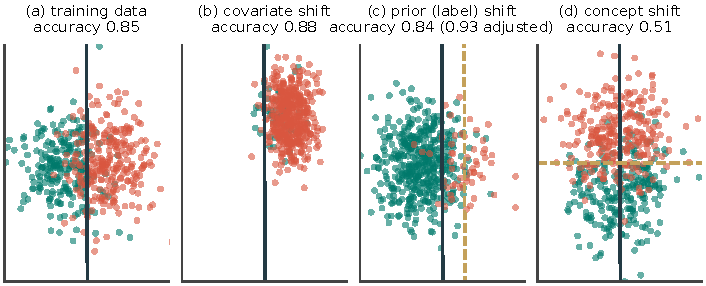
\includegraphics[width=\textwidth]{ch06/shift_types}
\caption{Types of dataset shift on a two-class problem. The solid line is the boundary of a logistic
regression trained on (a); the dashed lines are the boundary adapted to the new prior (c) and the new true
boundary (d). Titles give the accuracy of the original model.}
\label{fig:shifttypes}
\end{figure}

\paragraph{A causal view} Which type of shift is plausible depends on the causal direction of the problem
(\cref{sec:causality}) \citep{schoelkopf2012causal}. When the features cause the target ($X\rightarrow Y$, as
when the characteristics of a loan determine whether it is repaid), the mechanism $p(y\mid x)$ tends to be
stable and the distribution of the causes $p(x)$ is what changes: covariate shift. When the target causes the
features ($Y\rightarrow X$, as when a disease causes symptoms, or a digit causes the image a person writes), the
mechanism $p(x\mid y)$ is the stable part and the prevalence $p(y)$ changes: label shift. This is why label
shift is natural in diagnosis and covariate shift in prediction from causes; but these are hypotheses to
justify, not consequences guaranteed by the direction of the arrows, since stability depends on which
mechanisms actually change.

\paragraph{Patterns over time} Drift also differs in how it unfolds \citep{gama2014survey,webb2016characterizing}
(\cref{fig:driftpatterns}): \emph{sudden} drift replaces a concept by another at once (a new regulation);
\emph{gradual} drift alternates between the old and the new concept, with the new one becoming more frequent
(customers slowly adopting a new product); \emph{incremental} drift moves continuously through intermediate
concepts (a sensor that degrades); and \emph{recurring} drift brings back concepts seen before (seasons,
weekdays and weekends). Recurring concepts suggest keeping old models instead of discarding them.

\begin{figure}[htbp]
\centering
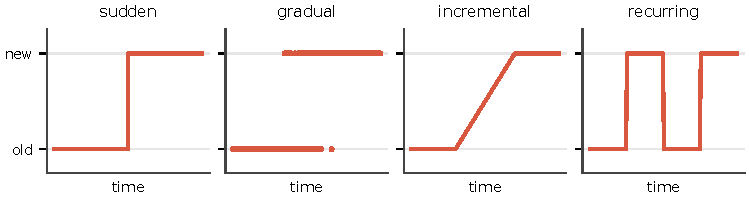
\includegraphics[width=\textwidth]{ch06/drift_patterns}
\caption{Four patterns of concept drift: which concept is active as time goes by.}
\label{fig:driftpatterns}
\end{figure}

% ---------------------------------------------------------------------
\section{Detecting shift}\label{sec:detectshift}

Shift can be detected with or without labels. Without labels we can only see changes in the inputs and in the
predictions, which may or may not affect performance; with labels we can watch the performance itself, but
labels usually arrive late.

\subsection{Without labels: data drift}

\paragraph{Univariate monitoring} The simplest approach compares the distribution of each feature in a
\emph{reference} window (for instance, the training data or the first month in production) with a
\emph{current} window. For numerical features, the two-sample \emph{Kolmogorov--Smirnov} test uses the largest
distance between the two empirical distribution functions, $D=\sup_x|F_{\text{ref}}(x)-F_{\text{cur}}(x)|$; for
categorical features, a $\chi^2$ test compares the frequencies. In credit scoring, the \emph{population
stability index} is a long-standing practice \citep{siddiqi2006credit}: with the proportions $e_i$ of the
reference data and $a_i$ of the current data in each of $B$ bins (usually the deciles of the reference),
\begin{equation}\label{eq:psi}
  \mathrm{PSI}=\sum_{i=1}^{B}\,(a_i-e_i)\,\ln\frac{a_i}{e_i},
\end{equation}
a symmetrised Kullback--Leibler divergence. Conventional thresholds read a PSI below 0.1 as no notable
change, between 0.1 and 0.25 as a moderate one and above 0.25 as a major one; they are conventions of the
index, not significance levels of a test. Its discretisation also has blind spots: a constant feature that
changes to another constant can fall in a single bin and give a PSI of 0, so constant, discrete and
missing values need their own checks.

\paragraph{Multivariate monitoring} Univariate monitors can miss changes in the \emph{relations} between
features. A general alternative is the \emph{domain classifier}, also known as a classifier two-sample test
\citep{lopezpaz2017revisiting}: label the reference examples 0 and the current ones 1, train a classifier, and
measure with cross-validation how well it separates them. An AUC close to 0.5 means that this classifier, with this sample,
cannot tell the two windows apart, which does not prove that their distributions are equal; higher values
indicate a detectable change, though neither a universal measure of distance nor, by themselves, a loss of
predictive performance, and the classifier itself
tells which features changed (through its feature importances, \cref{sec:agnostic}). For a suitable class of
classifiers, its accuracy is also related to the divergence between domains that appears in the bound on the
error of a model trained on one domain and used on the other \citep{bendavid2010theory}; the AUC of a particular
classifier is a diagnostic, not that divergence. Kernel two-sample tests based on the maximum mean discrepancy
\citep{gretton2012kernel}, which we met in \cref{sec:examplebased}, are another option.

\begin{pylisting}[label={lst:datadrift}]{Univariate tests, PSI and a domain classifier on five kinds of change}
import numpy as np
from scipy.stats import ks_2samp
from sklearn.ensemble import HistGradientBoostingClassifier
from sklearn.model_selection import cross_val_score

rng = np.random.default_rng(1)

def window(n=5000, shift=0.0, sd3=1.0, rho=0.8):
    """Three features; x1 and x2 correlated with coefficient rho."""
    cov = np.array([[1, rho, 0], [rho, 1, 0], [0, 0, sd3 ** 2]])
    return rng.multivariate_normal([shift, 0, 0], cov, n)

def psi(ref, cur, bins=10):
    """Population stability index over the deciles of the reference window."""
    edges = np.quantile(ref, np.linspace(0, 1, bins + 1))
    edges[0], edges[-1] = -np.inf, np.inf
    e = np.maximum(np.histogram(ref, edges)[0] / len(ref), 1e-6)
    a = np.maximum(np.histogram(cur, edges)[0] / len(cur), 1e-6)
    return float(np.sum((a - e) * np.log(a / e)))

def domain_auc(ref, cur):
    """Can a classifier tell the two windows apart? An AUC of 0.5 means no."""
    X = np.vstack([ref, cur])
    d = np.r_[np.zeros(len(ref)), np.ones(len(cur))]
    clf = HistGradientBoostingClassifier(max_iter=100, random_state=0)
    return cross_val_score(clf, X, d, cv=5, scoring="roc_auc").mean()

reference = window()
scenarios = {"no drift": window(), "mean of x1 +0.1 sd": window(shift=0.1),
             "mean of x1 +0.5 sd": window(shift=0.5), "sd of x3 x1.5": window(sd3=1.5),
             "correlation 0.8 -> -0.8": window(rho=-0.8)}
print("scenario                  max KS (min p)    max PSI   domain AUC")
for name, current in scenarios.items():
    ks = [ks_2samp(reference[:, j], current[:, j]) for j in range(3)]
    stat, p = max(k.statistic for k in ks), min(k.pvalue for k in ks)
    worst_psi = max(psi(reference[:, j], current[:, j]) for j in range(3))
    print(f"{name:24s}  {stat:.3f} ({p:7.1e})   {worst_psi:.3f}     "
          f"{domain_auc(reference, current):.3f}")
\end{pylisting}
\begin{pyoutput}
scenario                  max KS (min p)    max PSI   domain AUC
no drift                  0.020 (2.5e-01)   0.005     0.493
mean of x1 +0.1 sd        0.051 (4.0e-06)   0.013     0.515
mean of x1 +0.5 sd        0.203 (2.4e-90)   0.241     0.700
sd of x3 x1.5             0.107 (1.6e-25)   0.201     0.604
correlation 0.8 -> -0.8   0.025 (9.7e-02)   0.006     0.892
\end{pyoutput}

\Cref{lst:datadrift} compares the three monitors on windows of 5000 examples with three features, the first two
correlated. Without drift, all of them stay quiet. A shift of the mean of one feature by 0.1 standard deviations
is \emph{statistically significant} for the Kolmogorov--Smirnov test ($p=4\cdot10^{-6}$), but its PSI is 0.013 and
the domain classifier barely notices it (AUC 0.515): with large windows, tests detect changes too small to
matter, so their $p$-values must not be read as measures of importance. A shift of half a standard deviation is
caught by all of them (PSI 0.24, AUC 0.70), and so is a change of the variance of the third feature. But when the
correlation between the first two features changes from 0.8 to $-0.8$, leaving every marginal distribution
intact, the univariate tests see nothing (the smallest $p$-value is 0.097 and the largest PSI 0.006), while the
domain classifier separates the windows with an AUC of 0.892. Whether a model suffers depends on how it uses the
two features and on their relation with the target, which only an evaluation with outcomes can tell.

Some practical advice applies to all these monitors. Monitoring many features with many tests produces false
alarms by chance, so thresholds must account for multiple testing or be set from the variation observed in
periods known to be stable. In high dimensions, it is often more effective to monitor a few summaries: the
predictions of the model, a low-dimensional projection of the inputs, or the output of a domain classifier
\citep{rabanser2019failing}. And under label shift, the distribution of the predicted labels together with the
confusion matrix measured on validation data allows the new class proportions to be estimated without labels
\citep{lipton2018detecting}, a problem we return to in \cref{sec:labelshift}.

\subsection{With labels: concept drift}

When the true outcomes arrive, we can watch the errors of the model directly. Concept drift detectors monitor
the stream of errors and signal when its rate increases significantly
\citep{gama2014survey,lu2019learning}:
\begin{itemize}
  \item the \emph{drift detection method} (DDM, \citealp{gama2004learning}) treats the errors as Bernoulli
        trials. After $i$ examples, the error rate is $p_i$ with standard deviation
        $s_i=\sqrt{p_i(1-p_i)/i}$. The detector remembers the moment at which $p_i+s_i$ was smallest, with
        values $p_{\min}$ and $s_{\min}$, and enters a \emph{warning} level when $p_i+s_i>p_{\min}+2s_{\min}$
        and a \emph{drift} level when $p_i+s_i>p_{\min}+3s_{\min}$. The examples received since the warning
        are the natural training set for a new model;
  \item the \emph{Page--Hinkley test} \citep{page1954continuous}, a sequential test for a change in the mean,
        accumulates the deviation of each observation from the mean available at that moment,
        $m_t=m_{t-1}+x_t-\bar x_t-\delta$, where $\bar x_t$ is the mean of the first $t$ observations and
        $\delta$ the magnitude of change that is tolerated, and signals an increase when $m_t-\min_{j\leq t}m_j$
        exceeds a threshold $\lambda$ (this one-sided version watches increases of the error rate); the moment of the minimum
        estimates when the change began;
  \item ADWIN (adaptive windowing, \citealp{bifet2007learning}) keeps a window of recent examples and drops its
        oldest part whenever two sub-windows have significantly different means, so that the window grows
        while the concept is stable and shrinks when it changes.
\end{itemize}

\begin{pylisting}[label={lst:conceptdrift}]{Detecting concept drift with DDM and Page--Hinkley, from scratch}
import numpy as np
from sklearn.linear_model import LogisticRegression

rng = np.random.default_rng(2)
T = 6000
X = rng.normal(size=(T, 2))
t = np.arange(T)
angle = np.where(t < 2000, 0.0, np.pi / 2) + np.clip((t - 4000) / 1000, 0, 1) * np.pi / 3
y = ((X * np.c_[np.cos(angle), np.sin(angle)]).sum(axis=1) > 0).astype(int)
y = np.where(rng.random(T) < 0.1, 1 - y, y)       # 10% label noise
# the concept changes suddenly at t = 2000 and incrementally between t = 4000 and 5000

class DDM:
    """Drift detection method (Gama et al., 2004) on a stream of 0/1 errors."""
    def __init__(self, warning=2.0, drift=3.0, min_n=100):
        self.warning, self.drift, self.min_n = warning, drift, min_n
        self.reset()

    def reset(self):
        self.n, self.errors, self.best, self.p_min, self.s_min = 0, 0, np.inf, 0, 0
        self.warning_at = None

    def update(self, error, t):
        """Returns None, or the estimated start of the new concept when drift is found."""
        self.n += 1
        self.errors += error
        p = self.errors / self.n
        s = np.sqrt(p * (1 - p) / self.n)
        if self.n < self.min_n:
            return None
        if p + s < self.best:                       # the best moment seen so far
            self.best, self.p_min, self.s_min = p + s, p, s
        if p + s > self.p_min + self.drift * self.s_min:      # strict: errors needed
            return t if self.warning_at is None else self.warning_at
        if p + s > self.p_min + self.warning * self.s_min:
            self.warning_at = t if self.warning_at is None else self.warning_at
        else:
            self.warning_at = None                  # a false warning
        return None

class PageHinkley:
    """Page-Hinkley test for an increase in the mean of a stream."""
    def __init__(self, delta=0.01, threshold=20):
        self.delta, self.threshold = delta, threshold
        self.reset()

    def reset(self):
        self.n, self.mean, self.m, self.m_min, self.t_min = 0, 0.0, 0.0, 0.0, None

    def update(self, x, t):
        """Returns None, or the estimated change point when the test fires."""
        self.n += 1
        self.mean += (x - self.mean) / self.n
        self.m += x - self.mean - self.delta
        if self.t_min is None or self.m < self.m_min:
            self.m_min, self.t_min = self.m, t
        return self.t_min if self.m - self.m_min > self.threshold else None

def run(detector=None, window=None, start=500, refresh=50, cap=2000):
    """Prequential evaluation: predict each example, then learn its label. Every `refresh`
    examples the model is retrained on the last `window` examples or, with a detector,
    on the data since the last detected change (an adaptive window)."""
    model = LogisticRegression().fit(X[:start], y[:start])
    since, errors, alarms = 0, [], []
    for i in range(start, T):
        e = int(model.predict(X[i:i + 1])[0] != y[i])
        errors.append(e)
        refit = (i - start + 1) % refresh == 0
        if detector is not None:
            change = detector.update(e, i)
            if change is not None:
                alarms.append(i)
                detector.reset()
                since, refit = max(change, i - 100), True   # noisy estimate: bound it
        if refit and (window is not None or detector is not None):
            first = i + 1 - window if window else max(since, i + 1 - cap)
            first = min(first, i + 1 - 30)           # at least 30 examples
            if np.unique(y[first:i + 1]).size == 2:    # both classes needed to refit
                model = LogisticRegression().fit(X[first:i + 1], y[first:i + 1])
    return np.array(errors), alarms

results = {"static model": run(), "sliding window": run(window=300),
           "DDM": run(DDM()), "Page-Hinkley": run(PageHinkley())}
print("                  overall   t < 2000   2000-4000   4000-6000   alarms")
for name, (errors, alarms) in results.items():
    part = [1 - errors[a - 500:b - 500].mean() for a, b in [(500, 2000), (2000, 4000),
                                                           (4000, T)]]
    print(f"{name:18s} {1 - errors.mean():.3f}     {part[0]:.3f}      {part[1]:.3f}"
          f"       {part[2]:.3f}    {', '.join(map(str, alarms)) or '-'}")
\end{pylisting}
\begin{pyoutput}
                  overall   t < 2000   2000-4000   4000-6000   alarms
static model       0.533     0.874      0.514       0.295    -
sliding window     0.863     0.865      0.851       0.873    -
DDM                0.862     0.870      0.856       0.863    2046, 4568, 4707
Page-Hinkley       0.863     0.870      0.853       0.867    2040, 4442, 5248
\end{pyoutput}

\Cref{lst:conceptdrift} and \cref{fig:conceptdrift} simulate a stream of 6000 examples whose concept changes
suddenly at $t=2000$ (the boundary rotates by 90 degrees) and incrementally between $t=4000$ and 5000 (it rotates
continuously by another 60 degrees). The evaluation is \emph{prequential}: each example is first predicted and then used for
learning once its label arrives. Four strategies are compared: a static model, which falls to an accuracy of
0.51 after the sudden drift and 0.30 at the end; a sliding window, which retrains every 50 examples on the last
300; and two adaptive windows, which retrain every 50 examples on all the data since the last change detected by
DDM or by Page--Hinkley. Both detectors signal the sudden drift within 40 to 46 examples. In the stable period
the adaptive windows use more data than the sliding window and are slightly better (0.870 against 0.865); after
the sudden drift they recover slightly better too (0.856 and 0.853 against 0.851); during the incremental drift they
signal two changes each but lag behind the sliding window, which forgets continuously (0.863 and 0.867 against
0.873). Overall the three adaptive strategies are tied at 0.86, but only the detectors tell a person that
something changed, and when. An alarm signals a change in \emph{performance}: by itself it does not identify
a change of $p(y\mid x)$, which a covariate shift towards regions where the model is worse, problems with
the labels or changes in the predictor can also cause, and a change of concept that leaves the aggregated
error unchanged goes unnoticed.

\begin{figure}[htbp]
\centering
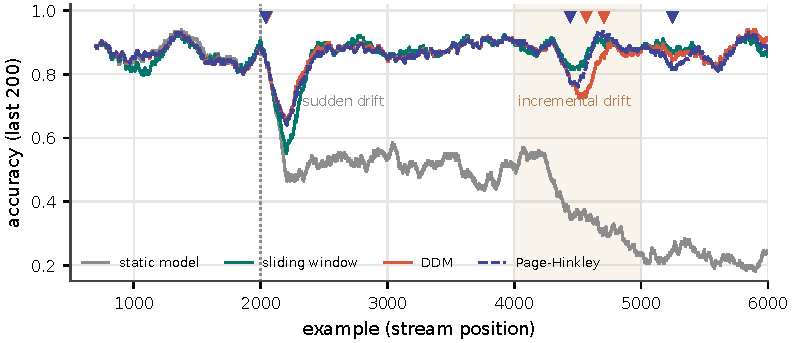
\includegraphics[width=\textwidth]{ch06/concept_drift}
\caption{Prequential accuracy (moving average of 200 examples) of four strategies on a stream with a sudden
drift at $t=2000$ and an incremental drift between $t=4000$ and 5000. Triangles mark the alarms of DDM and
Page--Hinkley.}
\label{fig:conceptdrift}
\end{figure}

\begin{pitfall}
The moment at which a change began is much harder to estimate than the fact that it happened. In a first version
of this experiment, the adaptive windows started at the beginning of the warning period of DDM or at the minimum
of the Page--Hinkley statistic; both were noisy and fell several hundred examples before the real change, so the
new models kept learning from the old concept, and the detectors did worse than a plain sliding window (0.80
against 0.86). Bounding how far back the new training data may start (here, 100 examples before the alarm) fixed
it. Detectors also raise false alarms, especially early on, when the minimum error rate is estimated from few
examples.
\end{pitfall}

% =====================================================================
\section{Adapting to shift}\label{sec:adapt}

Detecting shift is only useful if we can respond to it. The right response depends on the type of shift and on
the data available: labelled data from the new situation, unlabelled data only, or a few labels.

\subsection{Retraining strategies}

The most common response is to retrain the model with recent data. Several strategies are used in practice, often
combined \citep{gama2014survey,lu2019learning}:
\begin{itemize}
  \item \emph{periodic retraining} (every night, every week), simple and predictable, as in the continuous training
        pipeline of \cref{sec:infrastructure}; its period should match the speed at which the data change;
  \item \emph{triggered retraining}, when a monitor or a detector signals a change, which saves computation in
        stable periods and reacts quickly to sudden drift (\cref{lst:conceptdrift});
  \item \emph{windowing}: training only on the most recent data, with a fixed window or an adaptive one such as
        ADWIN; and \emph{weighting}, which keeps all the data but gives older examples less weight, for instance an
        exponentially decaying one;
  \item \emph{ensembles} that add models trained on recent data and remove or downweight those that perform poorly,
        which can also keep the models of recurring concepts (\cref{ch:hybrid});
  \item \emph{online learning}, which updates the model with each new example: stochastic gradient descent for
        linear models and neural networks, or Hoeffding trees for data streams \citep{domingos2000mining}.
\end{itemize}
Retraining requires labels. When they are scarce or delayed, the methods of the next subsections adapt a model using
unlabelled data from the new situation, provided we know which kind of shift has occurred.

\subsection{Correcting label shift and estimating class proportions}\label{sec:labelshift}

Under label shift the class-conditional distributions $p(x\mid y)$ are unchanged, so a probabilistic classifier
trained on the source can be corrected with Bayes' theorem once the new class priors are known: the new posterior is
proportional to the old one multiplied by the ratio of priors,
\begin{equation}\label{eq:priorcorrection}
  p_t(y\mid x)=\frac{\frac{\pi_t(y)}{\pi_s(y)}\,p_s(y\mid x)}{\sum_{y'}\frac{\pi_t(y')}{\pi_s(y')}\,p_s(y'\mid x)},
\end{equation}
where $\pi_s$ and $\pi_t$ are the class proportions in the source and in the target. The difficulty is that the new
proportions are unknown. Estimating them from unlabelled data is a learning task in its own right, called
\emph{quantification} \citep{forman2008quantifying,gonzalez2017review}. The main methods are:
\begin{itemize}
  \item \emph{classify and count} (CC): the proportion of examples that the classifier assigns to each class. It is
        biased, because the errors of the classifier do not cancel when the proportions change;
  \item \emph{adjusted classify and count} (ACC): corrects CC with the true and false positive rates of the
        classifier, estimated on the source by cross-validation: $\hat\pi=(\mathrm{CC}-\FPR)/(\TPR-\FPR)$;
  \item \emph{probabilistic classify and count} (PCC): the average predicted probability, which works when the
        probabilities are calibrated for the target, and its adjusted variants \citep{bella2010quantification};
  \item the \emph{EM algorithm} of \citet{saerens2002adjusting}: start with $\pi_t=\pi_s$, correct the posteriors with
        \cref{eq:priorcorrection}, re-estimate $\pi_t$ as the average corrected posterior, and repeat until convergence.
        It estimates the new priors and corrects the posteriors at the same time.
\end{itemize}
These corrections rest on assumptions: stable class-conditional distributions, an informative and stable
confusion matrix for ACC (it needs $\TPR\neq\FPR$, and a nearly singular matrix in the multiclass case makes it
unstable), and probabilities that represent the source posteriors for PCC and EM. When the counts are not
informative, ACC can even fall outside $[0,1]$ (with $\mathrm{CC}=0.05$, $\TPR=0.8$ and $\FPR=0.1$ it gives $-0.07$),
and such estimates must be reported as infeasible rather than silently clipped.

\begin{pylisting}[label={lst:labelshift}]{Estimating the new class proportions and correcting the posteriors}
import numpy as np
from sklearn.linear_model import LogisticRegression
from sklearn.metrics import brier_score_loss, log_loss
from sklearn.model_selection import cross_val_predict

rng = np.random.default_rng(3)
mu = np.array([1.0, 0.5, 0.0, -0.5, 0.8])          # how the positive class differs

def sample(n, prior):
    """Same class-conditional distributions p(x|y); only p(y) changes."""
    y = (rng.random(n) < prior).astype(int)
    return rng.normal(size=(n, 5)) + np.outer(y, mu), y

X_s, y_s = sample(5000, 0.5)                       # training data: balanced
model = LogisticRegression().fit(X_s, y_s)
X_t, y_t = sample(20000, 0.1)                      # deployment: 10% positives, no labels
p_t = model.predict_proba(X_t)[:, 1]

cc = np.mean(p_t >= 0.5)                           # classify and count
p_cv = cross_val_predict(LogisticRegression(), X_s, y_s, cv=5,
                         method="predict_proba")[:, 1]          # honest TPR and FPR
tpr, fpr = np.mean(p_cv[y_s == 1] >= 0.5), np.mean(p_cv[y_s == 0] >= 0.5)
acc = (cc - fpr) / (tpr - fpr)                     # adjusted classify and count
if not 0 <= acc <= 1:                              # not a valid prevalence: report it
    print(f"ACC = {acc:.3f} lies outside [0, 1]: the counts are not informative")
pcc = p_t.mean()                                   # probabilistic classify and count

def em_prior(p, prior_s, max_iter=1000, tol=1e-8):
    """Saerens et al. (2002): EM estimate of the new prior and of the posteriors."""
    prior = prior_s
    for _ in range(max_iter):                      # until the prior stops changing
        a = prior / prior_s * p
        post = a / (a + (1 - prior) / (1 - prior_s) * (1 - p))
        prior, old = post.mean(), prior
        if abs(prior - old) < tol:
            break
    return prior, post

em, post = em_prior(p_t, y_s.mean())
print(f"true prevalence {y_t.mean():.3f}; estimated: CC {cc:.3f}, ACC {acc:.3f}, "
      f"PCC {pcc:.3f}, EM {em:.3f}")
for name, q in [("unadjusted model", p_t), ("adjusted by EM", post)]:
    print(f"{name:17s} accuracy {np.mean((q >= 0.5) == y_t):.3f}   "
          f"Brier {brier_score_loss(y_t, q):.4f}   log loss {log_loss(y_t, q):.4f}")
\end{pylisting}
\begin{pyoutput}
true prevalence 0.106; estimated: CC 0.284, ACC 0.099, PCC 0.352, EM 0.104
unadjusted model  accuracy 0.771   Brier 0.1560   log loss 0.4761
adjusted by EM    accuracy 0.906   Brier 0.0724   log loss 0.2484
\end{pyoutput}

\Cref{lst:labelshift} trains a logistic regression on balanced data and deploys it where only 10.6\% of the examples
are positive. Classify and count estimates 28.4\% and probabilistic classify and count 35.2\%, both far off, because
the classifier was trained for a world with 50\% positives. The adjusted count (9.9\%) and EM (10.4\%) are close to the
truth. Correcting the posteriors with the prior estimated by EM, without a single label from the new situation, raises
the accuracy from 0.771 to 0.906 and halves the Brier score and the log loss (\cref{sec:scoring}).

\subsection{Correcting covariate shift}

Under covariate shift $p(y\mid x)$ is unchanged, so why should a model trained on the source fail? If the model can
represent the true relationship and has enough data everywhere, it does not, as \cref{fig:shifttypes}b showed. But
models are always approximations, and training spends their capacity on the regions where the \emph{training} data are
dense, which may not be where the deployment data are. The remedy is \emph{importance weighting}
\citep{shimodaira2000improving}: the expected loss on the target can be written as an expectation on the source,
\begin{equation}
  \E_{(x,y)\sim p_t}\bigl[\ell(f(x),y)\bigr]=\E_{(x,y)\sim p_s}\bigl[w(x)\,\ell(f(x),y)\bigr],\qquad
  w(x)=\frac{p_t(x)}{p_s(x)},
\end{equation}
so training on the source examples weighted by $w(x)$ fits the model where it will be used. The densities are unknown,
but their ratio can be estimated directly: by kernel mean matching \citep{huang2007correcting}, by KLIEP
\citep{sugiyama2008direct}, or, most simply, with a domain classifier that separates source from target inputs
\citep{bickel2009discriminative}: if it estimates the probability $q(x)$ that $x$ comes from the target, with $n_s$ source
and $n_t$ target examples,
\begin{equation}
  \hat w(x)=\frac{n_s}{n_t}\cdot\frac{q(x)}{1-q(x)} .
\end{equation}

\begin{pylisting}[label={lst:covshift}]{Importance weighting under covariate shift}
import numpy as np
from scipy.stats import norm
from sklearn.linear_model import LinearRegression, LogisticRegression

rng = np.random.default_rng(4)
f = lambda x: -x + x ** 3                              # the true regression function
x_s = rng.normal(0.5, 0.5, 200)                        # training inputs
y_s = f(x_s) + rng.normal(0, 0.3, 200)
x_t = rng.normal(0.0, 0.3, 1000)                       # deployment inputs
y_t = f(x_t) + rng.normal(0, 0.3, 1000)                # labels: evaluation and reference
col = lambda x: x.reshape(-1, 1)                       # a misspecified linear model

w_true = norm.pdf(x_s, 0, 0.3) / norm.pdf(x_s, 0.5, 0.5)    # p_target(x) / p_source(x)
both = np.r_[x_s, x_t]
is_target = np.r_[np.zeros(200), np.ones(1000)]
domain = LogisticRegression().fit(np.c_[both, both ** 2], is_target)
q = domain.predict_proba(np.c_[x_s, x_s ** 2])[:, 1]   # P(deployment | x)
w_est = 200 / 1000 * q / (1 - q)                       # the same ratio, from a classifier
fit = lambda x, y, w=None: LinearRegression().fit(col(x), y, sample_weight=w)
fits = {"unweighted": fit(x_s, y_s), "weighted (estimated w)": fit(x_s, y_s, w_est),
        "weighted (true w)": fit(x_s, y_s, w_true),
        "deployment fit (resubstitution)": fit(x_t, y_t)}
for name, m in fits.items():
    mse = np.mean((m.predict(col(x_t)) - y_t) ** 2)
    print(f"{name:32s} slope {m.coef_[0]:+.2f}   MSE on deployment data {mse:.3f}")
ess = lambda w: w.sum() ** 2 / (w ** 2).sum()          # effective sample size
print(f"effective sample size: {ess(w_est):.0f} (estimated w), {ess(w_true):.0f} (true w)"
      " of 200")
\end{pylisting}
\begin{pyoutput}
unweighted                       slope +0.46   MSE on deployment data 0.285
weighted (estimated w)           slope -0.57   MSE on deployment data 0.091
weighted (true w)                slope -0.59   MSE on deployment data 0.091
deployment fit (resubstitution)  slope -0.73   MSE on deployment data 0.089
effective sample size: 76 (estimated w), 79 (true w) of 200
\end{pyoutput}

\Cref{lst:covshift} and \cref{fig:covshift} reproduce the classic example of \citet{shimodaira2000improving}: the true
function is a cubic, the model is a straight line, and the training inputs are centred at 0.5 while the deployment inputs
are centred at 0 with a smaller spread. The ordinary least-squares line fits the training region, where the cubic rises
(slope $+0.46$), and has an error of 0.285 on the deployment data. Weighting by the true density ratio, or by the ratio
estimated with a logistic domain classifier, fits the region where the model will be used (slope $-0.57$) and divides the
error by three (0.091), almost the 0.089 of a line fitted to the deployment data themselves and scored on the same data, a
resubstitution reference rather than an estimate of generalisation.

\begin{figure}[htbp]
\centering
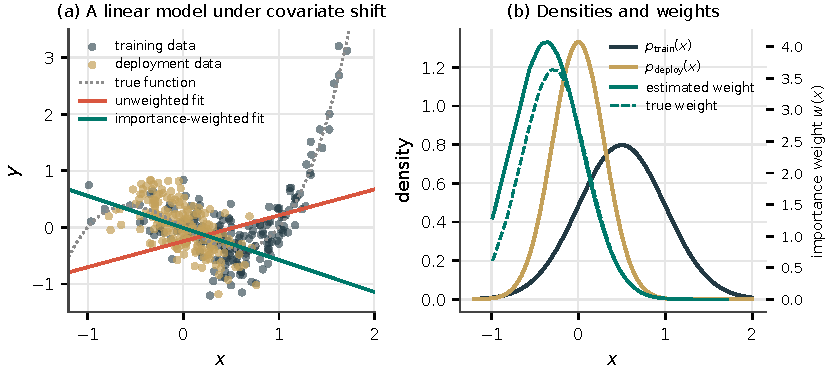
\includegraphics[width=\textwidth]{ch06/covariate_shift}
\caption{Covariate shift. (a) Training and deployment data, the true function, and linear fits without and with
importance weights. (b) The two input densities and the importance weights, true and estimated with a domain
classifier.}
\label{fig:covshift}
\end{figure}

Importance weighting has a price. A few training examples with large weights dominate the fit, which increases the
variance: the \emph{effective sample size}, $(\sum_iw_i)^2/\sum_iw_i^2$, is only 76 of the 200 training examples in the
listing. And the method fails completely where the target has data but the source has none, since no weight can create
information that was never collected: importance weighting needs the support of the target to be covered by the source.
Flattening the weights (raising them to a power between 0 and 1) or clipping them trades bias for variance.

\subsection{Domain adaptation and transfer learning}\label{sec:transfer}

\emph{Domain adaptation} is the general problem of using a model trained in a source domain in a different but related
target domain, with few or no labels in the target; \emph{transfer learning} extends it to related but different tasks
\citep{pan2010survey}. A classic result bounds the error of a model $h$ on the target by its error on the source, plus a
measure of the divergence between the input distributions of the two domains, plus the error of the best model on both
domains together \citep{bendavid2010theory}:
\begin{equation}
  \varepsilon_t(h)\leq\varepsilon_s(h)+\tfrac12\,d_{\mathcal H\Delta\mathcal H}(\mathcal D_s,\mathcal D_t)+\lambda^\star .
\end{equation}
The divergence can be estimated, for a given class of classifiers, with a domain classifier, as in
\cref{lst:datadrift}, and the bound suggests the main families of methods: reduce the divergence by changing
how the data are represented, and keep the source error low. Aligning the inputs is not enough when
$\lambda^\star$ is large: if $p(x)$ is the same in both domains but $y_s=\mathbb 1[x>0]$ and $y_t=\mathbb 1[x<0]$, the
inputs are indistinguishable and the perfect source model is always wrong on the target.
\begin{itemize}
  \item \emph{instance-based} methods reweight or select source examples so that they resemble the target, as
        importance weighting does;
  \item \emph{feature-based} methods map both domains into a representation where they look alike. CORAL
        \citep{sun2016return} aligns the second-order statistics: it whitens the source features with their covariance
        $C_s$ and recolours them with the target covariance $C_t$, $\tilde X_s=(X_s-\mu_s)\,C_s^{-1/2}C_t^{1/2}+\mu_t$, and
        then trains on the transformed source. Domain-adversarial neural networks \citep{ganin2016domain} learn a
        representation that predicts the target well while a domain classifier fails to tell the domains apart;
  \item \emph{parameter-based} methods transfer what a model has learned. With a few target labels, the source model can
        be fine-tuned on them, or a target model can be trained with a penalty that keeps it close to the source model,
        $\min_w\,L_t(w)+\lambda\|w-w_s\|^2$ \citep{chelba2006adaptation}. \emph{Feature augmentation}
        \citep{daume2007frustratingly} triplicates the features into a shared copy and a copy for each domain,
        $\Phi_s(x)=(x,x,0)$ and $\Phi_t(x)=(x,0,x)$, and trains one model on both domains, which learns what is common and
        what is specific to each.
\end{itemize}
Deep learning made transfer the default: the first layers of a network trained on a large data set learn general
features that can be reused for other tasks \citep{yosinski2014transferable}, and today many applications start from a
large pre-trained \emph{foundation model} and adapt it with a few examples or a little fine-tuning
\citep{bommasani2021opportunities}. Transfer can also hurt: when the domains are too different, using the source makes the
target model worse (\emph{negative transfer}), so the transferred model must always be compared with one trained on the
target data alone.

\begin{pylisting}[label={lst:coral}]{Unsupervised domain adaptation with CORAL}
import numpy as np
from scipy.linalg import sqrtm
from sklearn.datasets import make_classification
from sklearn.linear_model import LogisticRegression
from sklearn.model_selection import cross_val_score, train_test_split

X, y = make_classification(n_samples=6000, n_features=10, n_informative=6, random_state=5)
X_s, X_t, y_s, y_t = train_test_split(X, y, test_size=0.5, random_state=0)
rng = np.random.default_rng(5)
gain = np.diag(rng.uniform(0.5, 2.0, 10))                  # recalibrated sensors...
mix = np.eye(10) + 0.3 * rng.normal(size=(10, 10))              # ...with cross-talk
X_t = X_t @ gain @ mix + rng.normal(0, 1, 10)                    # ...and offsets

def coral(X_s, X_t, eps=1.0):
    """CORAL (Sun et al., 2016): give the source the mean and (regularised) covariance of
    the target, approximately."""
    I = np.eye(X_s.shape[1])
    C_s, C_t = np.cov(X_s, rowvar=False) + eps * I, np.cov(X_t, rowvar=False) + eps * I
    recolour = np.real(np.linalg.inv(sqrtm(C_s)) @ sqrtm(C_t))   # whiten, then colour
    return (X_s - X_s.mean(0)) @ recolour + X_t.mean(0)

standardise = lambda Z: (Z - Z.mean(0)) / Z.std(0)
model = lambda: LogisticRegression(max_iter=2000)
print(f"no adaptation             {model().fit(X_s, y_s).score(X_t, y_t):.3f}")
per_domain = model().fit(standardise(X_s), y_s).score(standardise(X_t), y_t)
print(f"standardise each domain   {per_domain:.3f}")
print(f"CORAL                     {model().fit(coral(X_s, X_t), y_s).score(X_t, y_t):.3f}")
print(f"with target labels (CV)   {cross_val_score(model(), X_t, y_t, cv=5).mean():.3f}")
\end{pylisting}
\begin{pyoutput}
no adaptation             0.618
standardise each domain   0.615
CORAL                     0.724
with target labels (CV)   0.841
\end{pyoutput}

\Cref{lst:coral} simulates a common industrial situation: the sensors of a machine are replaced, and the new ones have
different gains and offsets and some cross-talk between channels. A classifier trained on the old sensors has an
accuracy of 0.618 on the new ones. Standardising each domain separately, which corrects the gains and offsets, does not
help (0.615), because the cross-talk mixes the features. CORAL, which needs only unlabelled data from the new sensors,
raises the accuracy to 0.724, well above doing nothing but well below the 0.841 that labelled data from the new sensors
would allow: aligning two moments cannot undo every transformation. With the regularisation of the listing
(a constant added to both covariances), CORAL matches the regularised moments only approximately; and it
uses all the unlabelled target inputs, a legitimate transductive protocol when they are available, whose
moments must be frozen or updated explicitly for new data.

\begin{pylisting}[label={lst:transferlearning}]{Transfer with few target labels: five strategies}
import numpy as np
from scipy.optimize import minimize
from sklearn.linear_model import LogisticRegression

rng = np.random.default_rng(6)
d = 20
w_source = rng.normal(size=d)                       # plenty of labelled data for this one
w_target = w_source + rng.normal(0, 0.5, d)         # a related concept, with few labels

def task(w, n):
    X = rng.normal(size=(n, d))
    return X, (rng.random(n) < 1 / (1 + np.exp(-(X @ w)))).astype(int)

X_s, y_s = task(w_source, 3000)
X_test, y_test = task(w_target, 5000)
LR = lambda: LogisticRegression(fit_intercept=False, max_iter=2000)
w0 = LR().fit(X_s, y_s).coef_[0]
zeros = lambda X: np.zeros_like(X)
augment = lambda X, target: np.c_[X, zeros(X), X] if target else np.c_[X, X, zeros(X)]

def towards_source(X, y, lam=5.0):
    """Logistic regression regularised towards the source weights (parameter transfer)."""
    def loss(w):
        z = X @ w
        return np.mean(np.logaddexp(0, z) - y * z) + lam * np.sum((w - w0) ** 2) / len(y)
    return minimize(loss, w0, method="L-BFGS-B").x

accuracy = lambda w: np.mean(((X_test @ w) > 0) == y_test)
methods = ["target", "source", "pooled", "augmented", "regularised"]
curves = {m: [] for m in methods}
sizes = [10, 20, 50, 100, 200, 500]
for n in sizes:
    scores = {m: [] for m in methods}
    for _ in range(10):
        X_t, y_t = task(w_target, n)
        while y_t.min() == y_t.max():
            X_t, y_t = task(w_target, n)
        scores["target"].append(accuracy(LR().fit(X_t, y_t).coef_[0]))
        scores["source"].append(accuracy(w0))
        pooled = LR().fit(np.r_[X_s, X_t], np.r_[y_s, y_t]).coef_[0]
        scores["pooled"].append(accuracy(pooled))
        aug = LR().fit(np.r_[augment(X_s, False), augment(X_t, True)], np.r_[y_s, y_t])
        scores["augmented"].append(np.mean(aug.predict(augment(X_test, True)) == y_test))
        scores["regularised"].append(accuracy(towards_source(X_t, y_t)))
    for m in methods:
        curves[m].append(np.mean(scores[m]))
print("target labels" + "".join(f"{m:>13s}" for m in methods))
for i, n in enumerate(sizes):
    print(f"{n:13d}" + "".join(f"{curves[m][i]:13.3f}" for m in methods))
\end{pylisting}
\begin{pyoutput}
target labels       target       source       pooled    augmented  regularised
           10        0.649        0.849        0.849        0.819        0.853
           20        0.720        0.849        0.850        0.821        0.854
           50        0.779        0.849        0.850        0.802        0.857
          100        0.831        0.849        0.851        0.836        0.863
          200        0.860        0.849        0.852        0.860        0.870
          500        0.872        0.849        0.855        0.872        0.875
\end{pyoutput}

\Cref{lst:transferlearning} and \cref{fig:transfer} study the case with a few labels. A source task has 3000 labelled
examples; a related target task, whose weights differ from those of the source by random perturbations, has between 10
and 500. Training on the target labels alone needs between 100 and 200 of them to match the source model used as it is (0.849).
Pooling both data sets barely moves away from the source model, because the source examples dominate. Feature augmentation
pays off only with enough target data: with 10 to 50 labels the target-specific copies of the features overfit and the
model is worse than the source model (0.80 to 0.82), and it becomes competitive from 200 labels. Regularising the target
model towards the source weights has the highest mean accuracy at every size in this task and these ten
repetitions, from 0.853 with 10 labels to 0.875 with 500: it starts
from what the source knows and moves only as far as the target data justify.

\begin{figure}[htbp]
\centering
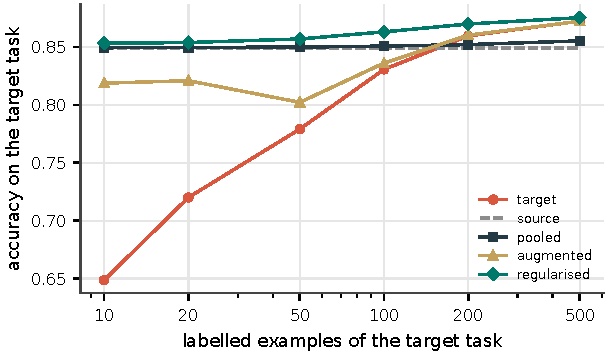
\includegraphics[width=0.75\textwidth]{ch06/transfer}
\caption{Accuracy on a target task as a function of the number of its labelled examples, for a model trained on the
target only, the source model, a model trained on both, feature augmentation, and a target model regularised towards the
source (mean of 10 repetitions).}
\label{fig:transfer}
\end{figure}

% =====================================================================
\section{Monitoring applications built on large language models}\label{sec:llmmonitor}

The applications of \cref{sec:llmapps} need monitoring as much as any other model, and three features make it harder.
Their outputs are free text, which cannot be compared with a label as simply as a class can. Their inputs are open: users
can ask anything, in any language and in any way. And when the model is used through an API, it can change without
notice, because the provider updates it. The levels of \cref{fig:monitorlayers} still apply, with new metrics at each of
them.

\paragraph{Operational metrics} Besides the latency of the whole answer, interactive applications track the \emph{time to
the first token}, which determines how responsive they feel. The number of tokens per request and per user determines the
cost, and must be watched like any other expense: a prompt that grows by accident, or a loop in an agent, can multiply the
bill. Errors, timeouts and rate limits of the provider, and the share of answers served from a cache, complete the picture.

\paragraph{Quality without labels} Most answers are never checked by anybody, so quality is estimated indirectly. Users give
\emph{explicit feedback} (a thumbs up or down) and \emph{implicit feedback}: rephrasing the same question, abandoning the
conversation or asking for a human are signs of a bad answer. A random sample of conversations can be reviewed by people, and
a larger one by a language model acting as a judge, provided that its ratings have first been compared with those of people on
the same sample (\cref{sec:llmapps}). For RAG applications, the share of the claims of each answer that are supported by the
retrieved passages measures its \emph{groundedness}, and the share of questions for which the assistant abstains measures the
gaps in its knowledge: a rising abstention rate means that users are asking about something the index does not cover.

\paragraph{Drift of the questions} What users ask changes: a new product, a news story, a change in the season or an outage
bring new topics, and with them questions the application was not designed or tested for. The methods of \cref{sec:detectshift}
apply directly to text. \Cref{lst:querydrift} represents the questions to a bank's assistant with TF-IDF, as in \cref{lst:rag},
and trains a domain classifier to distinguish the questions of a reference week from those of the current one.

\begin{pylisting}[label={lst:querydrift}]{Detecting drift in the questions asked to an assistant}
import numpy as np
from sklearn.feature_extraction.text import TfidfVectorizer
from sklearn.linear_model import LogisticRegression
from sklearn.model_selection import cross_val_score

rng = np.random.default_rng(19)
TOPICS = {   # what users ask a bank's assistant, by topic
 "balance": ["what is my balance", "how much money do I have", "show my last movements",
             "why is my balance lower than expected"],
 "card": ["my card was blocked", "how do I activate my new card", "card payment declined",
          "I lost my card"],
 "transfer": ["how do I make a transfer", "transfer not received", "cancel a transfer",
              "transfer limit per day"],
 "mortgage": ["mortgage interest rate", "can I repay my mortgage early",
              "documents for a mortgage"],
 "login": ["I cannot log in", "reset my access code", "the app does not open"],
 "bizum": ["how do I send money with bizum", "bizum payment not received",
           "bizum limit per day", "register my phone in bizum"],   # a new service
}
EXTRAS = ["", "please", "hello", "urgent", "thanks", "again", "today"]

def week(n, mix):
    topics, probs = list(mix), np.array(list(mix.values())) / sum(mix.values())
    out = []
    for t in rng.choice(topics, n, p=probs):
        out.append(f"{rng.choice(EXTRAS)} {rng.choice(TOPICS[t])} {rng.choice(EXTRAS)}")
    return out

usual = {"balance": 30, "card": 25, "transfer": 25, "mortgage": 10, "login": 10}
launch = dict(usual, bizum=15)                 # the bank launches instant payments
reference = week(3000, usual)
print("current week compared with the reference   domain AUC   most typical words now")
for name, current in [("same topics", week(3000, usual)),
                      ("new service launched", week(3000, launch))]:
    tfidf = TfidfVectorizer()
    X = tfidf.fit_transform(reference + current)
    d = np.r_[np.zeros(len(reference)), np.ones(len(current))]
    auc = cross_val_score(LogisticRegression(max_iter=1000), X, d, cv=5,
                          scoring="roc_auc").mean()
    coef = LogisticRegression(max_iter=1000).fit(X, d).coef_[0]
    top = tfidf.get_feature_names_out()[np.argsort(-coef)[:3]]
    print(f"{name:40s}   {auc:8.3f}     {', '.join(top) if auc > 0.55 else '-'}")
\end{pylisting}
\begin{pyoutput}
current week compared with the reference   domain AUC   most typical words now
same topics                                   0.507     -
new service launched                          0.573     bizum, with, send
\end{pyoutput}

When the current week has the same mix of topics as the reference, the domain classifier cannot tell them apart (AUC 0.507). When
the bank launches an instant payment service and 15\% of the questions ask about it, the AUC rises to 0.573: a modest value, because
85\% of the questions are as usual, but enough to raise an alert, and the words on which the classifier relies say what changed:
\emph{bizum}, \emph{send} and \emph{with}, from questions such as ``how do I send money with Bizum''. The knowledge base of the
assistant must be extended, and its test set (\cref{sec:llmapps}) with it, before users start receiving invented answers.

\paragraph{Changes in the model} When a provider updates a model behind an API, the behaviour of the application can change from
one day to the next. A study of two widely used models found that their behaviour on several tasks, from solving mathematical
problems to generating code, changed substantially between versions released only three months apart \citep{chen2024chatgpt}. The
defences are those of \cref{sec:safedeploy}: pin the version of the model whenever the provider allows it, run the regression test
set before adopting a new version, and roll it out gradually, in shadow mode or with a canary, comparing the old and new answers on
real traffic.

\paragraph{Safety and security} Applications that talk to the public must also be monitored for abuse: attempts at prompt
injection and at making the model ignore its instructions, leaks of personal data in the answers, and harmful content. Each of
them needs an alert, a person responsible and a procedure to respond. Under the AI Act, chatbots must tell users that they are
talking to a machine, and the providers of high-risk systems must monitor them after deployment and report serious incidents
(\cref{sec:aiact}).

\begin{pitfall}
An assistant that answers fluently is not necessarily answering correctly. Monitoring only the operational metrics of a language
model application (it is fast, cheap and never fails) can hide that its answers have become wrong, because a wrong answer looks
exactly like a right one. Some measure of quality, however indirect, must be part of the dashboard.
\end{pitfall}

% =====================================================================
\section{Deploying updates safely}\label{sec:safedeploy}

Continuous integration and delivery make it easy to release new versions quickly; the challenge is to obtain
evidence, under declared criteria, that they are better. For machine learning, a suite of tests is not enough: a new model can pass every test, beat the
old one on held-out data, and still be worse in production. There is no substitute for live performance, but exposing
users to a worse model has a cost. The usual solution is to move a new model through stages that give progressively
more information at progressively more risk (\cref{fig:rollout}).

\begin{figure}[htbp]
\centering
\begin{tikzpicture}[font=\scriptsize\sffamily,
  st/.style={draw=edmnavy,fill=edmnavy!6,rounded corners=2pt,minimum height=11mm,minimum width=22mm,align=center},
  arr/.style={-{Stealth[length=1.8mm]},edmnavy}]
  \node[st] (a) at (0,0) {offline\\evaluation\\(test data)};
  \node[st] (b) at (2.75,0) {shadow mode\\(predictions\\logged, not used)};
  \node[st] (c) at (5.5,0) {canary\\(a small share\\of users)};
  \node[st] (d) at (8.25,0) {A/B test\\(randomised\\groups)};
  \node[st] (e) at (11.0,0) {full rollout\\(and continued\\monitoring)};
  \foreach \x/\y in {a/b,b/c,c/d,d/e} \draw[arr] (\x) -- (\y);
  \draw[-{Stealth[length=2.2mm]},edmcoral,thick] (-1.1,0.95) -- node[above] {risk for the users} (12.1,0.95);
  \draw[-{Stealth[length=2.2mm]},edmteal,thick] (-1.1,-0.95) -- node[below] {information about the real impact} (12.1,-0.95);
\end{tikzpicture}
\caption{Stages for deploying a new model, from the safest to the most informative.}
\label{fig:rollout}
\end{figure}

\subsection{Why offline evaluation is not enough}

The test data of \cref{ch:evaluation} answer the question ``how good would this model have been on past data?''.
Production asks a different one, and the answers differ for several reasons. The test data are already old when the
model is deployed, and the world may have drifted (\cref{sec:shift}). The features computed in production may differ
from those used in training, because they are computed by different code, from different sources, or with different
delays: this \emph{training--serving skew} is one of the most common causes of failures in production, and it
goes unnoticed by an offline evaluation that uses only the training pipeline, unless the features produced by
the serving path are tested against those of training \citep{breck2019data}. The model's own actions change the data it will see next (a feedback loop).
And users react to a new model in ways that no historical data set can show: a recommender that is more accurate
offline may be less engaging, because it recommends what users would have found anyway.

\subsection{Shadow mode}

In \emph{shadow mode} the new model is deployed in parallel to the existing one: both compute their predictions for
every request and both are logged, but the application uses only those of the existing model. Shadow mode lets
engineers check, on real production traffic and without changing the user experience:
\begin{itemize}
  \item that the infrastructure copes with the new model: latency, memory, failures;
  \item how often the two models agree, and where they disagree (by segment, by input range);
  \item whether the distribution of the new predictions is plausible (the share of each decision, the range of the
        scores);
  \item and, once outcomes arrive, how accurate the new model is on the cases whose representative labels
        are available: if the current policy decides which outcomes are observed (only granted loans are
        repaid or not), the evaluation inherits that selection, and a holdout or a counterfactual design is
        needed.
\end{itemize}
The cost is double computation, and care is needed with side effects: the shadow model must never write to shared
state, send messages or update the features of other models. And one thing shadow mode cannot show is how users
respond to the new model, because they never see its outputs.

\begin{pylisting}[label={lst:shadow}]{Shadow mode catches a training--serving skew}
import numpy as np
from sklearn.ensemble import GradientBoostingClassifier
from sklearn.linear_model import LogisticRegression

rng = np.random.default_rng(10)

def applicants(n):
    income = rng.normal(30, 8, n)                    # thousand EUR
    debt, age = rng.uniform(0, 0.8, n), rng.integers(18, 80, n)
    logit = 0.12 * (income - 30) - 4 * (debt - 0.4) + 0.03 * (age - 45)
    y = (rng.random(n) < 1 / (1 + np.exp(-logit))).astype(int)
    return np.c_[income, debt, age], y

X_train, y_train = applicants(5000)
X_test, y_test = applicants(5000)
# in production
current = LogisticRegression(max_iter=1000).fit(X_train[:, :2], y_train)
candidate = GradientBoostingClassifier(random_state=0).fit(X_train, y_train)
print(f"offline accuracy: current {current.score(X_test[:, :2], y_test):.3f}, "
      f"candidate {candidate.score(X_test, y_test):.3f}")

X_live, y_live = applicants(20000)                   # a week of real requests
served = current.predict(X_live[:, :2])              # what the users receive
X_feed = X_live.copy()
# bug: the new feature service sends EUR
X_feed[:, 0] *= 1000
shadow = candidate.predict(X_feed)                   # computed and logged, never used
print(f"shadow week: agreement {np.mean(served == shadow):.3f}, approval rate "
      f"current {served.mean():.3f}, candidate {shadow.mean():.3f}")
print(f"once the outcomes arrive: current {np.mean(served == y_live):.3f}, "
      f"candidate {np.mean(shadow == y_live):.3f}")
fixed = candidate.predict(X_live)                    # after fixing the units
print(f"after the fix: agreement {np.mean(served == fixed):.3f}, "
      f"candidate accuracy {np.mean(fixed == y_live):.3f}")
\end{pylisting}
\begin{pyoutput}
offline accuracy: current 0.715, candidate 0.727
shadow week: agreement 0.641, approval rate current 0.534, candidate 0.872
once the outcomes arrive: current 0.712, candidate 0.585
after the fix: agreement 0.887, candidate accuracy 0.726
\end{pyoutput}

\Cref{lst:shadow} shows shadow mode catching a typical skew. The candidate, a gradient boosting model with one more
feature, beats the current model offline (0.727 against 0.715). In production, its new feature service sends the income
in euros instead of thousands of euros. During the shadow week the two models agree on only 64\% of the applicants, and
the candidate would approve 87\% of them against 53\% for the current model: a red flag long before any outcome is known.
When the outcomes arrive, the candidate's accuracy is 0.585 (the simulation knows the outcome of every
applicant, which a real bank would not). After the units are fixed, the agreement rises to 89\% and
the candidate's production accuracy (0.726) matches its offline estimate. Had it been deployed directly, every user
would have received the decisions of a broken model.

\subsection{Canary releases and progressive rollout}

A \emph{canary release} serves the new model to a small share of the users (often 1\%) and increases the share in stages,
as long as \emph{guardrail} metrics show no harm: technical ones (error rate, latency) and business ones (conversion,
complaints). If a guardrail is violated, the rollout stops and the previous version is restored automatically. Two practices
make this fast and safe: \emph{blue--green} deployments keep the previous version running, so that switching back is
instantaneous, and \emph{feature flags} turn a model on or off for chosen users without a new deployment. Every deployed
model should be a registered, versioned artefact, so that any earlier version can be redeployed
(\cref{sec:infrastructure}).

\begin{pylisting}[label={lst:canary}]{A progressive rollout with guardrails and automatic rollback}
import numpy as np
from scipy.stats import fisher_exact

rng = np.random.default_rng(11)
STAGES = [0.01, 0.05, 0.20, 0.50, 0.95]   # share of requests for the new model;
DAILY = 100_000                           # 5% stay on the old one as a control
BASE = {"conversion": 0.050, "errors": 0.001}        # the current model

def worse(events_new, n_new, events_old, n_old, higher_is_better, alpha=0.01):
    """Exact one-sided test of harm (Fisher), suitable for rare events such as errors."""
    table = [[events_new, n_new - events_new], [events_old, n_old - events_old]]
    side = "less" if higher_is_better else "greater"
    return fisher_exact(table, alternative=side).pvalue < alpha

def rollout(model):
    exposed = 0
    for share in STAGES:                             # one day of requests per stage
        n_new = int(DAILY * share)
        n_old = DAILY - n_new
        exposed += n_new
        for metric, better in [("errors", False), ("conversion", True)]:   # guardrails
            e_new = rng.binomial(n_new, model[metric])
            e_old = rng.binomial(n_old, BASE[metric])
            if worse(e_new, n_new, e_old, n_old, better):
                return (f"rolled back at {share:.0%} ({metric}), "
                        f"{exposed:,} requests served")
    return f"passed every stage, {exposed:,} requests served during the rollout"

for name, model in [("good model", {"conversion": 0.052, "errors": 0.001}),
                    ("crashes more", {"conversion": 0.050, "errors": 0.020}),
                    ("converts less", {"conversion": 0.046, "errors": 0.001})]:
    print(f"{name:14s} {rollout(model)}")
false = np.mean(["rolled" in rollout(BASE) for _ in range(2000)])
print(f"an identical model is rolled back in {false:.1%} of 2000 rollouts "
      "(10 tests at the 1% level)")
\end{pylisting}
\begin{pyoutput}
good model     passed every stage, 171,000 requests served during the rollout
crashes more   rolled back at 1% (errors), 1,000 requests served
converts less  rolled back at 5% (conversion), 6,000 requests served
an identical model is rolled back in 6.7% of 2000 rollouts (10 tests at the 1% level)
\end{pyoutput}

\Cref{lst:canary} rolls out three candidates through five stages (1\%, 5\%, 20\%, 50\% and 95\% of a day's requests,
keeping 5\% on the old model as a real control until the end), comparing each guardrail with the current model by
an exact one-sided test, suitable for rare events such as errors. A good model goes through. A model that fails 2\%
of its requests is stopped at the first stage, after 1000 requests. In this run, a model whose conversion rate is 4.6\%
instead of 5.0\% is stopped at 5\%, after 6000 requests; but at such small stages a difference like that is detected
only occasionally, and \emph{the absence of an alarm is not evidence that a model is not worse}. The tests have their own
price: with ten tests at the 1\% level, an identical model is rolled back in 6.7\% of the rollouts. A real rollout plan
fixes in advance the acceptable harm, how the budget of false alarms is spread across stages and metrics, and the
evidence required to advance. Canaries catch large problems quickly; to measure small differences reliably we need
a properly designed experiment.

% =====================================================================
\section{A/B testing and experimentation}\label{sec:abtesting}

The principle of an \emph{A/B test}, or online controlled experiment, is simple: expose a random sample of the users to the new
model (the treatment, B) and the rest to the current one (the control, A); after enough time, compare a metric between the groups
and keep the better model \citep{kohavi2009controlled,kohavi2020trustworthy}. Randomisation is what makes the comparison causal
(\cref{sec:causality}): because users are assigned to groups by chance, the groups differ, on average, only in the model they
receive. \Cref{fig:abanatomy} shows the parts of an experimentation system.

\begin{figure}[htbp]
\centering
\begin{tikzpicture}[font=\scriptsize\sffamily,
  st/.style={draw=edmnavy,fill=edmnavy!6,rounded corners=2pt,minimum height=12mm,minimum width=21mm,align=center},
  arr/.style={-{Stealth[length=1.6mm]},edmnavy}]
  \node[st] (u) at (0,0) {request\\from a user};
  \node[st] (h) at (2.45,0) {assignment\\$\mathrm{hash}(\text{salt},\text{id})$\\$\rightarrow$ A or B};
  \node[st] (m) at (4.9,0) {model A\\or model B};
  \node[st] (l) at (7.35,0) {event logs\\(exposures,\\clicks, \dots)};
  \node[st] (k) at (9.8,0) {metrics\\per group};
  \node[st,fill=edmgold!20] (a) at (12.25,0) {analysis: SRM\\check, intervals,\\decision};
  \foreach \x/\y in {u/h,h/m,m/l,l/k,k/a} \draw[arr] (\x) -- (\y);
\end{tikzpicture}
\caption{The anatomy of an online experiment.}
\label{fig:abanatomy}
\end{figure}

\subsection{Designing the experiment}

An experiment starts with a hypothesis (``the new ranking model increases the purchases per user'') and with decisions that must
be taken before it starts:
\begin{itemize}
  \item the \emph{randomisation unit}: usually the user, so that each person has a consistent experience; sessions or requests
        give more units but break consistency, and in marketplaces or social networks, where users influence each other,
        groups of connected users or periods of time may have to be randomised instead;
  \item the \emph{metrics}: one main metric, or overall evaluation criterion, that defines success and that the change is expected
        to move; \emph{guardrail} metrics that must not get worse (latency, errors, revenue, unsubscriptions); and \emph{invariant}
        metrics that the treatment should not affect beyond sampling variation, the first of which is the share of users
        in each group;
  \item the \emph{groups}: users in both groups should be as similar as possible, so that any difference in the outcome can be
        attributed to the model and not to a difference between cohorts (if group A contained all the heavy users and group B only
        occasional ones, the experiment would be inconclusive), which randomisation achieves; the treatment group must be large
        enough to detect the effect, but as small as possible to limit the exposure to a potentially worse model;
  \item the \emph{duration}: long enough to reach the planned sample size, in whole weeks to average out weekly cycles, and long
        enough for \emph{novelty} and \emph{primacy} effects (users reacting to the change itself) to fade; too long, and users may
        be lost. Effects that take months to appear, such as changes in retention, are measured with long-term holdout groups
        \citep{hohnhold2015focusing}.
\end{itemize}

\subsection{Assigning users and checking the assignment}

The simplest infrastructure stores the group of each user with the rest of their information, and lets the system decide which
model serves each request; this works well when users are logged in. Equivalently, and without storage, a user can be assigned by
hashing their identifier together with an experiment-specific \emph{salt}: the same user always gets the same variant, and
different salts make the assignments of different experiments independent, which is what allows large companies to run many
experiments at the same time on the same users \citep{tang2010overlapping}. Independent assignment does not stop the
interventions themselves from interacting when two experiments change the same part of the product, which platforms
handle with layers of mutually exclusive experiments. Experiments assume that each user is exposed to only
one variant, an assumption broken if users see several (for instance on different devices); identifying anonymous users with
cookies or network addresses requires more infrastructure and is less reliable.

The first analysis of any experiment is a sanity check of the assignment. A \emph{sample ratio mismatch} (SRM), a split of users
between the groups significantly different from the intended one, means that something is broken: a variant that crashes for some
users and loses their logs, a redirect that drops users, a bot filter that acts differently on each variant. An SRM alarm calls
for an investigation before the results can be trusted, however good they look \citep{fabijan2019diagnosing}; like any
test it has false alarms, and the absence of an SRM does not certify the rest of the logging.

\begin{pylisting}[label={lst:srm}]{Hash-based assignment and the sample ratio mismatch check}
import hashlib
import numpy as np
from scipy.stats import chisquare

def variant(user, experiment, share_b=0.5):
    """Deterministic assignment: hash the user with an experiment-specific salt."""
    digest = hashlib.sha256(f"{experiment}:{user}".encode()).hexdigest()
    return "B" if int(digest[:8], 16) / 16 ** 8 < share_b else "A"

users = [f"user{i}" for i in range(100_000)]
first = np.array([variant(u, "new-ranker") for u in users])
second = np.array([variant(u, "new-colours") for u in users])
print("same user, same variant every time:", variant("user42", "new-ranker") == first[42])
both_b = np.mean((first == "B") & (second == "B"))
print(f"share in B in both experiments: {both_b:.3f} (independent: 0.250)")

def srm(n_a, n_b, share_b=0.5):
    """Sample ratio mismatch: do the observed counts match the intended split?"""
    total = n_a + n_b
    return chisquare([n_a, n_b], [total * (1 - share_b), total * share_b]).pvalue

alarm = lambda p: "SRM alarm" if p < 0.001 else "no alarm"   # strict: run on every test
n_a, n_b = np.sum(first == "A"), np.sum(first == "B")
p = srm(n_a, n_b)
print(f"logged users A {n_a:,}, B {n_b:,}: p-value {p:.4f}, {alarm(p)}")
lost = int(0.02 * n_b)                    # a bug in B loses 2% of its users' logs
p = srm(n_a, n_b - lost)
print(f"with 2% of B's logs lost: B {n_b - lost:,}, p-value {p:.1e}, {alarm(p)}")
\end{pylisting}
\begin{pyoutput}
same user, same variant every time: True
share in B in both experiments: 0.248 (independent: 0.250)
logged users A 50,423, B 49,577: p-value 0.0075, no alarm
with 2% of B's logs lost: B 48,586, p-value 5.3e-09, SRM alarm
\end{pyoutput}

\Cref{lst:srm} assigns 100,000 users to two experiments by hashing: assignments are consistent, and 24.8\% of the users are in
group B of both experiments, as expected from independent 50/50 splits. The SRM check is a $\chi^2$ test of the observed counts
against the intended split. Because it is run on every experiment, it uses a strict threshold, typically 0.001: the correct
assignment gives $p=0.0075$, no alarm, while losing the logs of 2\% of the users of B gives $p=5\cdot10^{-9}$, a clear alarm.

\subsection{Estimating the better variant}

Most A/B tests compare a metric such as the click-through rate. Deciding which variant is better is more than choosing the group
with the higher rate: the difference must be statistically significant, which for two proportions is usually checked with a
two-sample $z$-test (\cref{sec:stats}),
\begin{equation}
  z=\frac{\hat p_B-\hat p_A}{\sqrt{\hat p\,(1-\hat p)\,\bigl(\frac1{n_A}+\frac1{n_B}\bigr)}},
\end{equation}
where $\hat p$ is the pooled rate. The amount of data needed depends on the rate and on the size of the change to be detected, the
\emph{minimum detectable effect}, and it must be decided \emph{before} the test starts. To detect a change from $p_1$ to $p_2$ with
significance level $\alpha$ and power $1-\beta$, each group needs approximately
\begin{equation}\label{eq:samplesize}
  n=\frac{\Bigl(z_{1-\alpha/2}\sqrt{2\bar p(1-\bar p)}+z_{1-\beta}\sqrt{p_1(1-p_1)+p_2(1-p_2)}\Bigr)^2}{(p_2-p_1)^2},
  \qquad \bar p=\frac{p_1+p_2}{2},
\end{equation}
users. Small effects on small rates need large samples: to detect an increase of the CTR from 5.0\% to 5.5\% with $\alpha=0.05$ and a
power of 0.8, each group needs 31,234 users (\cref{lst:abtest}). The formula assumes one independent opportunity (a click or not) per
user. When users are randomised but each one contributes several impressions, those are not independent, and the
uncertainty of a click-through rate must be computed at the level of users, for instance with a bootstrap over users or
the delta method \citep{deng2018applying}; counting logged events as if they were users overstates the evidence.

\begin{pylisting}[label={lst:abtest}]{Sample size, z-test and the cost of peeking at an A/B test}
import numpy as np
from scipy.stats import norm

def sample_size(p1, p2, alpha=0.05, power=0.8):
    """Users per group to detect a change from p1 to p2 with a two-sided z-test."""
    z_a, z_b = norm.ppf(1 - alpha / 2), norm.ppf(power)
    p = (p1 + p2) / 2
    num = z_a * np.sqrt(2 * p * (1 - p)) + z_b * np.sqrt(p1 * (1 - p1) + p2 * (1 - p2))
    return int(np.ceil(num ** 2 / (p2 - p1) ** 2))

def z_test(clicks_a, n_a, clicks_b, n_b):
    """Two-proportion z-test; works element-wise on arrays."""
    pa, pb = clicks_a / n_a, clicks_b / n_b
    p = (clicks_a + clicks_b) / (n_a + n_b)
    z = (pb - pa) / np.sqrt(p * (1 - p) * (1 / n_a + 1 / n_b))
    return z, 2 * norm.sf(np.abs(z))

n = sample_size(0.050, 0.055)
print(f"users per group to detect a CTR of 5.5% against 5.0%: {n:,}")
rng = np.random.default_rng(7)
a, b = rng.binomial(n, 0.050), rng.binomial(n, 0.055)
z, p = z_test(a, n, b, n)
print(f"one experiment: CTR A {a / n:.4f}, CTR B {b / n:.4f}, z = {z:.2f}, p = {p:.4f}")

looks, reps = 20, 5000                       # A/A tests: no real difference at all
seg = n // looks
users = seg * np.arange(1, looks + 1)
end = peek = 0
for _ in range(reps):
    ca = np.cumsum(rng.binomial(seg, 0.05, looks))
    cb = np.cumsum(rng.binomial(seg, 0.05, looks))
    p = z_test(ca, users, cb, users)[1]
    end += p[-1] < 0.05                       # one test at the planned end
    peek += np.any(p < 0.05)                  # stop as soon as anything looks significant
print(f"false positives in A/A tests: {end / reps:.3f} testing once, "
      f"{peek / reps:.3f} peeking {looks} times")
\end{pylisting}
\begin{pyoutput}
users per group to detect a CTR of 5.5% against 5.0%: 31,234
one experiment: CTR A 0.0498, CTR B 0.0537, z = 2.18, p = 0.0289
false positives in A/A tests: 0.044 testing once, 0.235 peeking 20 times
\end{pyoutput}

The result should be reported as an effect with a confidence interval, not only as a $p$-value: a significant difference may be too
small to matter, and a non-significant one may hide an important effect that the test was too small to detect. When several metrics or
several variants are compared, the chance of a false positive grows with the number of comparisons, and corrections such as Holm's
(\cref{sec:stats}) or a control of the false discovery rate are needed. And results that look too good deserve extra suspicion:
surprising effects in online experiments are more often bugs than discoveries \citep{kohavi2020trustworthy}.

\subsection{Reducing the variance}

The variance of the metric determines how many users an experiment needs. Much of that variance has nothing to do with the treatment:
some users simply use the product more than others. \emph{CUPED} \citep{deng2013improving} removes the part of the variance that can be
predicted from data collected \emph{before} the experiment, such as each user's activity in the previous weeks. With $X$ the pre-experiment
metric and $Y$ the metric during the experiment, it analyses
\begin{equation}
  Y^{\mathrm{cv}}=Y-\theta\,(X-\bar X),\qquad \theta=\frac{\operatorname{cov}(X,Y)}{\operatorname{var}(X)},
\end{equation}
whose mean difference between the groups estimates the same effect, because $X$ was measured before the assignment and cannot be affected by
it, but whose variance is smaller by a factor $1-\rho^2$, where $\rho$ is the correlation between $X$ and $Y$.

\begin{pylisting}[label={lst:cuped}]{Variance reduction with pre-experiment data (CUPED)}
import numpy as np

rng = np.random.default_rng(13)
n = 20_000                                            # users per group
def group(effect):
    # activity score in the month before the test
    before = rng.gamma(2.0, 2.5, n)
    during = 1.0 + 0.8 * before + rng.normal(0, 2.0, n) + effect
    return before, during

xa, ya = group(0.0)
xb, yb = group(0.1)                                   # B adds 0.1 to the activity score
x, y = np.r_[xa, xb], np.r_[ya, yb]
theta = np.cov(x, y)[0, 1] / np.var(x, ddof=1)        # CUPED: Y - theta (X - mean X)
adj = lambda xs, ys: ys - theta * (xs - x.mean())

def summary(a, b):
    diff = b.mean() - a.mean()
    se = np.sqrt(a.var(ddof=1) / n + b.var(ddof=1) / n)
    return diff, 1.96 * se

for name, (a, b) in [("plain difference", (ya, yb)),
                     ("CUPED", (adj(xa, ya), adj(xb, yb)))]:
    diff, half = summary(a, b)
    print(f"{name:17s} effect {diff:+.3f} +/- {half:.3f}   (95% CI)")
rho = np.corrcoef(x, y)[0, 1]
print(f"correlation before/during {rho:.2f}: variance and sample size reduced by "
      f"{rho ** 2:.0%}")
\end{pylisting}
\begin{pyoutput}
plain difference  effect +0.114 +/- 0.068   (95% CI)
CUPED             effect +0.097 +/- 0.039   (95% CI)
correlation before/during 0.82: variance and sample size reduced by 67%
\end{pyoutput}

In \cref{lst:cuped} the correlation between the sessions of each user before and during the experiment is 0.82, so CUPED removes 67\% of
the variance: the 95\% confidence interval of the effect shrinks from $\pm0.068$ to $\pm0.039$ sessions per user, and an experiment would
need a third of the users for the same power.

\subsection{Peeking and sequential tests}

A frequent error is to check the significance continuously and declare the test successful as soon as a significant result appears. Each look
is another chance for noise to cross the threshold, so the real false positive rate is much higher than the nominal one. In
\cref{lst:abtest}, with A/A tests in which both groups receive the same model, testing once at the planned end produces 4.4\% false
positives, close to the nominal 5\%, while looking 20 times and stopping at the first significant result produces 23.5\%; with 100 looks it
reaches 37\% (\cref{fig:experimentation}a).

Looking at the data is not wrong; looking with the wrong threshold is. \emph{Group sequential designs}, developed for clinical trials, plan
a number of looks in advance and use stricter thresholds at each one, so that the overall false positive rate stays at $\alpha$. The
\emph{Pocock} design uses the same threshold at every look \citep{pocock1977group}; the \emph{O'Brien--Fleming} design uses very strict
thresholds at the beginning, which relax towards the end, so that the final test is almost the ordinary one
\citep{obrien1979multiple}; and \emph{alpha spending} functions allow the number and timing of the looks to be flexible
\citep{lan1983discrete}. Methods that give ``always valid'' $p$-values, which can be monitored continuously, are used by commercial
experimentation platforms \citep{johari2017peeking}.

\begin{pylisting}[label={lst:sequential}]{Calibrating group sequential boundaries by simulation}
import numpy as np

rng = np.random.default_rng(14)
K, SIMS = 5, 200_000                                  # five equally spaced looks

def z_paths(drift):
    """z statistics at the K looks; `drift` is the expected z at the final look."""
    steps = rng.normal(drift / np.sqrt(K), 1.0, (SIMS, K))
    return np.cumsum(steps, axis=1) / np.sqrt(np.arange(1, K + 1))

def calibrate(shape, alpha=0.05):
    """Scale a boundary shape so that the overall false positive rate is alpha."""
    null = np.abs(z_paths(0.0))
    lo, hi = 1.0, 6.0
    for _ in range(40):
        c = (lo + hi) / 2
        lo, hi = (c, hi) if np.mean((null > c * shape).any(axis=1)) > alpha else (lo, c)
    return hi * shape

looks = np.arange(1, K + 1)
designs = {"fixed (one test)": np.r_[np.full(K - 1, np.inf), 1.96],
           "Pocock": calibrate(np.ones(K)),
           "O'Brien-Fleming": calibrate(np.sqrt(K / looks))}
null, alt = np.abs(z_paths(0.0)), np.abs(z_paths(1.96 + 0.8416))   # 80% power if fixed
print("design             boundaries at the 5 looks          FPR    power   mean n")
for name, bound in designs.items():
    cross = alt > bound
    stop = np.where(cross.any(axis=1), cross.argmax(axis=1) + 1, K)
    bounds = " ".join(f"{b:5.2f}" if np.isfinite(b) else "    -" for b in bound)
    print(f"{name:17s}  {bounds}   {np.mean((null > bound).any(axis=1)):.3f}  "
          f"{cross.any(axis=1).mean():.3f}   {stop.mean() / K:.0%}")
\end{pylisting}
\begin{pyoutput}
design             boundaries at the 5 looks          FPR    power   mean n
fixed (one test)       -     -     -     -  1.96   0.051  0.799   100%
Pocock              2.41  2.41  2.41  2.41  2.41   0.051  0.711   71%
O'Brien-Fleming     4.55  3.22  2.63  2.28  2.04   0.050  0.789   80%
\end{pyoutput}

\Cref{lst:sequential} calibrates both designs by simulation for five looks. The Pocock threshold is 2.41 at every look; the O'Brien--Fleming
thresholds are 4.55, 3.22, 2.63, 2.28 and 2.04. Both keep the false positive rate at 5\%. With an effect that the single final test would
detect with a power of 0.80, the Pocock design stops earlier on average (it uses 71\% of the maximum sample) but loses power (0.71), while
O'Brien--Fleming keeps almost all of the power (0.79) and still saves 20\% of the users (\cref{fig:sequential}). These boundaries are calibrated for the stated Gaussian
process, five equally spaced looks and a two-sided rule; another schedule of looks or another metric requires
recalibrating them, and the reported rates are Monte Carlo estimates.

\begin{figure}[htbp]
\centering
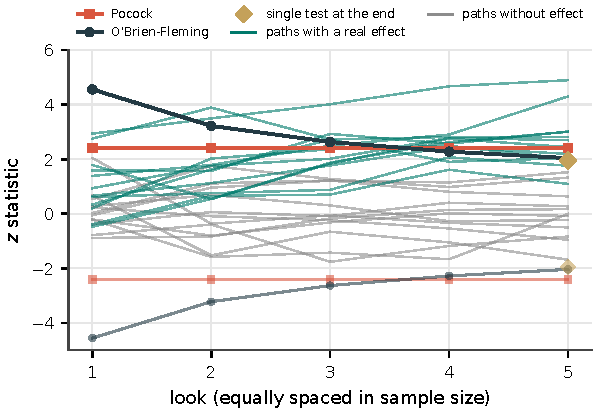
\includegraphics[width=0.72\textwidth]{ch06/sequential}
\caption{Group sequential boundaries for five looks (the test is two-sided: the lower boundaries mirror the upper
ones), with simulated $z$ paths with and without a real effect. A test stops at the first
look at which its path crosses the boundary.}
\label{fig:sequential}
\end{figure}

\subsection{A Bayesian view}

Some teams prefer to report the results of an experiment as probabilities about the variants rather than as $p$-values. With a uniform prior,
the click-through rate of each variant has a Beta posterior, $\mathrm{Beta}(1+\text{clicks},\,1+\text{non-clicks})$, and by drawing from
both posteriors we can estimate the probability that B is better than A, a credible interval for the relative lift, and the \emph{expected
loss} of choosing each variant, the clicks per user we would lose if it were in fact the worse one. A common decision rule is to choose a
variant once its expected loss is below a small threshold.

\begin{pylisting}[label={lst:bayesab}]{Posterior probability, lift and expected loss of an A/B test}
import numpy as np

# the experiment of the z-test listing
rng = np.random.default_rng(7)
n = 31_234
clicks_a, clicks_b = rng.binomial(n, 0.050), rng.binomial(n, 0.055)
draws = np.random.default_rng(15)
# Beta(1 + clicks, 1 + non-clicks): posterior of each CTR with a uniform prior
pa = draws.beta(1 + clicks_a, 1 + n - clicks_a, 200_000)
pb = draws.beta(1 + clicks_b, 1 + n - clicks_b, 200_000)
print(f"clicks A {clicks_a}, B {clicks_b} of {n:,} users each")
print(f"P(CTR of B > CTR of A) = {np.mean(pb > pa):.3f}")
lift = pb / pa - 1
lo, hi = np.percentile(lift, [2.5, 97.5])
print(f"relative lift: {np.median(lift):+.1%}, "
      f"95% credible interval [{lo:+.1%}, {hi:+.1%}]")
for choice, loss in [("A", np.maximum(pb - pa, 0)), ("B", np.maximum(pa - pb, 0))]:
    print(f"expected loss if we choose {choice}: {loss.mean():.5f} clicks per user")
\end{pylisting}
\begin{pyoutput}
clicks A 1557, B 1678 of 31,234 users each
P(CTR of B > CTR of A) = 0.986
relative lift: +7.8%, 95% credible interval [+0.8%, +15.2%]
expected loss if we choose A: 0.00388 clicks per user
expected loss if we choose B: 0.00001 clicks per user
\end{pyoutput}

For the experiment of \cref{lst:abtest} (\cref{lst:bayesab}), the probability that B is better is 0.986, the lift is $+7.8\%$ with a 95\%
credible interval from $+0.8\%$ to $+15.2\%$, and choosing B risks an expected loss of only 0.00001 clicks per user, against 0.00388 for A.
These numbers are easier to communicate than a $p$-value of 0.029, but they rest on the same data. Checking them repeatedly does not invalidate the posterior itself, given an adequate
prior and model, but a decision rule applied at every look does not inherit a given frequentist error rate.

\subsection{Evaluating new models offline from logs}

Every A/B test costs traffic and time, so teams try to discard bad candidates before testing them online. For ranking models,
\emph{interleaving} mixes the results of two rankers in a single list and counts which one's results the user clicks, which detects
differences with far fewer users than an A/B test \citep{chapelle2012large}. More generally, \emph{off-policy evaluation} estimates how a
new decision policy would have performed from the logs of the current one. This requires \emph{support}:
every action that the new policy may choose must have a positive probability under the current policy in that
context, and those probabilities (the \emph{propensities}) must be logged. Randomised logging policies provide it;
deterministic logs can only evaluate the decisions they cover. The \emph{inverse propensity scoring} estimator
\citep{horvitz1952generalization,li2011unbiased} averages, over the logged events, the reward of the events in which the logged action is
the one the new policy would have chosen, divided by the probability with which the current policy chose it:
\begin{equation}
  \hat V(\pi)=\frac1n\sum_{i=1}^{n}\frac{\mathbb 1[a_i=\pi(x_i)]\,r_i}{p(a_i\mid x_i)} .
\end{equation}
For a stochastic new policy, the indicator is replaced by the probability $\pi(a_i\mid x_i)$ that it chooses the logged
action; the estimate refers to the immediate reward, and the policy must be fixed before looking at the logs used to
evaluate it. Doubly robust estimators combine it with a model of the rewards: they remain consistent if either the
propensities or the reward model is correct, and often have lower variance \citep{dudik2011doubly}.

\begin{pylisting}[label={lst:ips}]{Off-policy evaluation of a new recommendation policy}
import numpy as np

rng = np.random.default_rng(16)
# rows: user segment, columns: article
ctr = np.array([[0.05, 0.04, 0.03],
                [0.09, 0.05, 0.04],
                [0.03, 0.04, 0.07]])
segment_share = np.array([0.5, 0.3, 0.2])
logging = np.array([[0.6, 0.2, 0.2],                 # the current, randomised policy
                    [0.6, 0.2, 0.2],
                    [0.2, 0.2, 0.6]])
n = 200_000
s = rng.choice(3, n, p=segment_share)
a = (rng.random(n)[:, None] > np.cumsum(logging[s], axis=1)).sum(axis=1)
r = (rng.random(n) < ctr[s, a]).astype(float)         # the logs: segment, article, click
new = np.array([1, 0, 2])                            # the policy we want to evaluate

truth = np.sum(segment_share * ctr[np.arange(3), new])
match = a == new[s]
naive = r[match].mean()                              # logged events where both agree
terms = match * r / logging[s, a]                    # inverse propensity scoring
ips, se = terms.mean(), terms.std() / np.sqrt(n)
print(f"CTR of the logging policy: {r.mean():.4f}")
print(f"new policy: true CTR {truth:.4f}, naive estimate {naive:.4f}, "
      f"IPS {ips:.4f} +/- {1.96 * se:.4f}")
print(f"the estimates use the {match.sum():,} logged events in which the policies agree")
\end{pylisting}
\begin{pyoutput}
CTR of the logging policy: 0.0552
new policy: true CTR 0.0610, naive estimate 0.0722, IPS 0.0616 +/- 0.0018
the estimates use the 80,167 logged events in which the policies agree
\end{pyoutput}

In \cref{lst:ips}, the current policy shows three articles to three user segments at random, with probabilities that differ by segment. A
new policy would have a click-through rate of 0.0610. Simply averaging the clicks of the logged events in which the old policy happened
to choose what the new one would choose gives 0.0722, an 18\% overestimate, because those events over-represent the segments in which
the agreement was more likely. Weighting by the inverse propensities gives $0.0616\pm0.0018$, an unbiased estimate obtained without showing
the new policy to a single user. Logs of this kind, with their propensities, are also what is needed to evaluate a contextual bandit before deploying it.

% =====================================================================
\section{Multi-armed bandits}\label{sec:bandits}

An A/B test explores for a fixed time and then exploits the winner. \emph{Multi-armed bandits} interleave the two, continuously
\citep{lattimore2020bandit}. The name comes from a gambler facing a row of slot machines (``one-armed bandits'') with unknown payouts. At each
step $t$ we choose an arm $a_t$ (a variant) and receive a reward (a click); each arm $a$ has an unknown expected reward $\mu_a$. The goal is to
maximise the total reward, or equivalently to minimise the \emph{regret}, the expected reward lost by not always choosing the best arm,
\begin{equation}
  R_T=T\mu^\star-\sum_{t=1}^{T}\mu_{a_t},\qquad \mu^\star=\max_a\mu_a .
\end{equation}
The listings compute this \emph{pseudo-regret}, from the expected rewards of the chosen arms rather than the clicks
actually observed, averaged over repetitions.
Every strategy faces the \emph{exploration--exploitation} dilemma: serving the arm that looks best earns now, but trying the others is the
only way to discover whether one of them is better. For stationary bandits with fixed gaps
between the arms, no strategy that performs well on every instance of the problem can have a regret that grows more slowly
than the logarithm of $T$ \citep{lai1985asymptotically} (a strategy that always plays one arm has zero regret where that arm
is the best, and linear regret elsewhere). Good strategies achieve the logarithmic rate, while an A/B test with a fixed
exploration phase, or $\varepsilon$-greedy with a fixed $\varepsilon$, has a regret that grows linearly; explore-then-commit
with an exploration that grows suitably with the horizon can be logarithmic. The main strategies are:
\begin{itemize}
  \item \emph{$\varepsilon$-greedy}: serve the best arm so far, except with probability $\varepsilon$, when a random arm is served. Simple,
        but it explores forever, and as much the clearly bad arms as the promising ones;
  \item \emph{upper confidence bounds} (UCB1, \citealp{auer2002finite}): serve the arm with the highest optimistic estimate, its mean reward
        plus a bonus that shrinks as the arm is tried more, $\bar x_a+\sqrt{2\ln t/n_a}$ (``optimism in the face of uncertainty'');
  \item \emph{Thompson sampling} \citep{thompson1933likelihood,chapelle2011empirical,russo2018tutorial}: keep a posterior distribution for the
        reward of each arm (for click rates, a Beta distribution updated with the clicks and non-clicks), draw a value from each posterior,
        and serve the arm with the highest draw. Arms are served in proportion to the probability that they are the best, so exploration
        concentrates on the arms that might still win \citep{scott2010modern}.
\end{itemize}

\begin{pylisting}[label={lst:bandits}]{An A/B test, epsilon-greedy, Thompson sampling and UCB1 on three variants}
import numpy as np

rng = np.random.default_rng(8)
ctr = np.array([0.050, 0.055, 0.060])              # true click rates, unknown to us
T = 50_000

def ab_test(t, clicks, shows, explore=15_000):     # equal split, then the winner
    return t % 3 if t < explore else int(np.argmax(clicks / shows))

def epsilon_greedy(t, clicks, shows, eps=0.1):     # usually the best so far
    if shows.min() == 0 or rng.random() < eps:
        return int(rng.integers(3))
    return int(np.argmax(clicks / shows))

def thompson(t, clicks, shows):                    # a plausible CTR per variant
    return int(np.argmax(rng.beta(1 + clicks, 1 + shows - clicks)))

# optimism: mean plus an uncertainty bonus
def ucb(t, clicks, shows):
    if shows.min() == 0:
        return int(np.argmin(shows))
    return int(np.argmax(clicks / shows + np.sqrt(2 * np.log(t + 1) / shows)))

def run(policy):
    clicks, shows, regret = np.zeros(3), np.zeros(3), np.empty(T)
    lost = 0.0
    for t in range(T):
        arm = policy(t, clicks, shows)
        clicks[arm] += rng.random() < ctr[arm]
        shows[arm] += 1
        lost += ctr.max() - ctr[arm]               # expected clicks lost by this choice
        regret[t] = lost
    return regret, shows[2] / T

curves = {}
for name, policy in [("A/B test, then winner", ab_test),
                     ("epsilon-greedy", epsilon_greedy), ("Thompson sampling", thompson),
                     ("UCB1", ucb)]:
    runs = [run(policy) for _ in range(10)]
    curves[name] = np.mean([r[0] for r in runs], axis=0)      # mean regret over time
    print(f"{name:22s} clicks lost {np.mean([r[0][-1] for r in runs]):6.1f}   "
          f"traffic to the best variant {np.mean([r[1] for r in runs]):.2f}")
\end{pylisting}
\begin{pyoutput}
A/B test, then winner  clicks lost   97.0   traffic to the best variant 0.71
epsilon-greedy         clicks lost   84.5   traffic to the best variant 0.77
Thompson sampling      clicks lost   47.7   traffic to the best variant 0.85
UCB1                   clicks lost  206.7   traffic to the best variant 0.42
\end{pyoutput}

\Cref{lst:bandits} and \cref{fig:experimentation}b compare four ways of choosing among three variants with click rates of 5.0\%, 5.5\% and 6.0\%,
over 50,000 users. An A/B/C test that splits the first 15,000 users equally and then serves the observed winner loses 97 expected clicks with
respect to always serving the best variant, and sends 71\% of the traffic to it; $\varepsilon$-greedy loses 85 and sends 77\%; Thompson sampling
loses only 48 and sends 85\%. UCB1 is the worst of all (207 clicks lost, 42\% of the traffic to the best variant): its bonus is designed for
rewards anywhere in $[0,1]$, and with click rates around 5\% it dwarfs the differences between the arms, so UCB1 keeps exploring long after the
others have settled. Variants that adapt the bonus to the variance of the rewards fix this, but the lesson is general: the constants of a
bandit algorithm matter as much as its name. These rankings hold for these click rates, settings, horizon and ten
repetitions, not in general.

\begin{figure}[htbp]
\centering
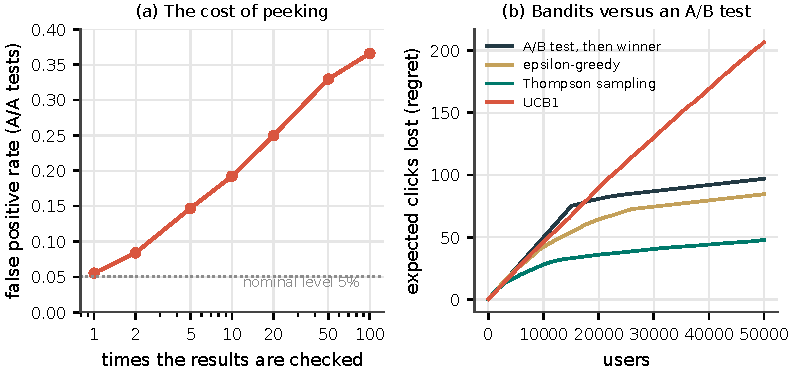
\includegraphics[width=\textwidth]{ch06/experimentation}
\caption{(a) False positive rate of A/A tests when the significance is checked repeatedly and the test stops at the first significant result.
(b) Expected clicks lost by an A/B test followed by the winner, $\varepsilon$-greedy, Thompson sampling and UCB1 (mean of 10 runs).}
\label{fig:experimentation}
\end{figure}

\subsection{When the world changes}

The strategies above assume that the reward of each arm is fixed. When it changes, as everything in this unit does, a bandit that has
accumulated a lot of evidence keeps trusting it: after thousands of plays, its posterior for the old best arm is so concentrated that it takes
a long time to notice that the arm has become the worst. The remedies are the same as for concept drift (\cref{sec:adapt}): forget old evidence,
by discounting it or by using only a sliding window of recent plays \citep{garivier2011upper}, or reset the bandit when a detector signals a
change.

\begin{pylisting}[label={lst:nsbandits}]{Thompson sampling with and without discounting when the best variant changes}
import numpy as np

rng = np.random.default_rng(17)
T, SWITCH = 40_000, 20_000
before = np.array([0.050, 0.055, 0.060])
after = np.array([0.060, 0.055, 0.045])              # the best variant becomes the worst

def run(discount):
    """Thompson sampling; with discount < 1, old evidence fades away."""
    clicks, shows, regret, lost = np.zeros(3), np.zeros(3), np.empty(T), 0.0
    for t in range(T):
        ctr = before if t < SWITCH else after
        arm = int(np.argmax(rng.beta(1 + clicks, 1 + shows - clicks)))
        clicks *= discount
        shows *= discount
        clicks[arm] += rng.random() < ctr[arm]
        shows[arm] += 1
        lost += ctr.max() - ctr[arm]
        regret[t] = lost
    return regret

curves = {}
for name, discount in [("Thompson", 1.0), ("discounted Thompson", 0.999)]:
    curves[name] = np.mean([run(discount) for _ in range(10)], axis=0)
    c = curves[name]
    print(f"{name:20s} clicks lost: {c[SWITCH - 1]:5.1f} before the change, "
          f"{c[-1] - c[SWITCH - 1]:6.1f} after it")
\end{pylisting}
\begin{pyoutput}
Thompson             clicks lost:  50.1 before the change,  161.6 after it
discounted Thompson  clicks lost:  77.5 before the change,   94.3 after it
\end{pyoutput}

In \cref{lst:nsbandits}, the best of three variants becomes the worst halfway through 40,000 users. Standard Thompson sampling loses 50 expected
clicks before the change and 162 after it, while it slowly unlearns the old winner. Discounting the evidence by a factor of 0.999 per play, which
keeps an effective memory of about 1000 plays in total (a half-life of about 700), costs more before the change (78 clicks, because it never becomes completely sure) but recovers much faster
(94 clicks after it), and loses less overall (\cref{fig:banditsadv}a).

\subsection{Contextual bandits}

The best variant is often not the same for every user. \emph{Contextual bandits} choose the variant from the features of the user and the
situation, learning a model of the reward of each arm as a function of the context \citep{li2010contextual}. LinUCB, for instance, fits a ridge
regression of the reward on the context $x$ for each arm, with parameters $\hat\theta_a=A_a^{-1}b_a$ (where $A_a$ accumulates $I+\sum xx^\top$ and
$b_a$ the reward-weighted contexts of the plays of arm $a$), and chooses the arm with the highest optimistic estimate,
\begin{equation}
  a_t=\argmax_a\Bigl(\hat\theta_a^\top x_t+\alpha\sqrt{x_t^\top A_a^{-1}x_t}\Bigr),
\end{equation}
whose bonus is large for contexts unlike those in which the arm has been tried.

\begin{pylisting}[label={lst:linucb}]{A contextual bandit (LinUCB) against a context-free one}
import numpy as np

rng = np.random.default_rng(18)
d, K, T = 5, 3, 20_000
# each variant appeals to different users
theta = rng.normal(0, 1, (K, d))

def ctr(x):
    """Click probability of each variant for a user with features x."""
    return 1 / (1 + np.exp(-(0.6 * theta @ x - 3.0)))

class LinUCB:
    """Li et al. (2010): a ridge regression per variant plus an optimism bonus."""
    def __init__(self, alpha=0.5):
        self.alpha = alpha
        self.A_inv = np.stack([np.eye(d + 1)] * K)
        self.b = np.zeros((K, d + 1))

    def choose(self, x):
        z = np.r_[x, 1.0]
        means = np.einsum("kij,kj,i->k", self.A_inv, self.b, z)
        bonus = np.sqrt(np.einsum("i,kij,j->k", z, self.A_inv, z))
        return int(np.argmax(means + self.alpha * bonus))

    def update(self, arm, x, reward):
        z = np.r_[x, 1.0]
        Az = self.A_inv[arm] @ z                       # Sherman-Morrison update
        self.A_inv[arm] -= np.outer(Az, Az) / (1 + z @ Az)
        self.b[arm] += reward * z

def simulate(policy):
    clicks, shows, lin, lost = np.zeros(K), np.zeros(K), LinUCB(), 0.0
    regret = np.empty(T)
    for t in range(T):
        x = rng.normal(size=d)
        p = ctr(x)
        if policy == "LinUCB":
            arm = lin.choose(x)
        elif policy == "Thompson (no context)":
            arm = int(np.argmax(rng.beta(1 + clicks, 1 + shows - clicks)))
        else:
            arm = int(np.argmax(p))                    # oracle: knows the click rates
        reward = float(rng.random() < p[arm])
        clicks[arm] += reward
        shows[arm] += 1
        lin.update(arm, x, reward)
        lost += p.max() - p[arm]
        regret[t] = lost
    return regret, clicks.sum() / T

results = {}
for policy in ["oracle", "Thompson (no context)", "LinUCB"]:
    regret, rate = simulate(policy)
    results[policy] = regret
    print(f"{policy:22s} CTR {rate:.4f}   expected clicks lost {regret[-1]:7.1f}")
\end{pylisting}
\begin{pyoutput}
oracle                 CTR 0.2019   expected clicks lost     0.0
Thompson (no context)  CTR 0.1289   expected clicks lost  1312.6
LinUCB                 CTR 0.1892   expected clicks lost    92.1
\end{pyoutput}

In \cref{lst:linucb} each of three variants appeals to different users. A context-free Thompson sampler finds the best variant on average and
reaches a click-through rate of 0.129; LinUCB, which uses five features of each user, reaches 0.189
(with a linear model that only approximates the logistic click rates of the simulation, in a single run), close to the 0.202 of an oracle that knows
the best variant for every user, and loses 92 expected clicks against 1313 (\cref{fig:banditsadv}b). Contextual bandits are a form of
personalisation that learns online. The LinUCB of the listing chooses by $\argmax$, deterministically, so its logs do not
support the off-policy evaluation of other policies (\cref{lst:ips}): that requires randomising part of the traffic, for
instance by exploring with a small probability, and logging the actual probability of each chosen action.

\begin{figure}[htbp]
\centering
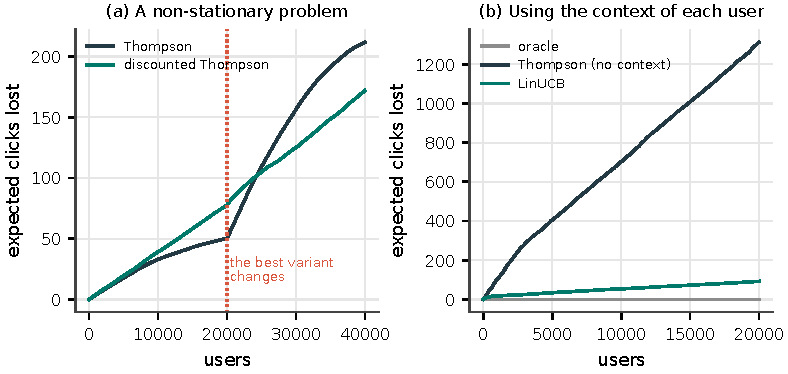
\includegraphics[width=\textwidth]{ch06/bandits_advanced}
\caption{(a) Expected clicks lost by Thompson sampling with and without discounting when the best variant changes. (b) A contextual bandit
(LinUCB) against a context-free one and an oracle (mean of 10 and 1 runs).}
\label{fig:banditsadv}
\end{figure}

\subsection{Bandits in practice}

Real deployments add complications. Rewards arrive with delays (a purchase days after a click), and models are updated in batches rather than
after every request, which reduces the advantage of adaptive allocation. The reward must be chosen carefully: optimising clicks can promote
sensational content at the expense of long-term satisfaction. Because the allocation adapts to the results, the plain averages of the rewards of
each arm are biased, so a bandit is a poor tool for estimating effect sizes. Bandits are the better choice when the goal is to earn while learning,
for short-lived decisions with many alternatives (headlines, creatives, promotions); A/B tests remain preferable when the goal is an unbiased
estimate of the effect of a change on many metrics, including slow ones such as retention. Several companies offer hosted experimentation and
optimisation services for organisations without a dedicated team.

% =====================================================================
\section{Summary}\label{sec:summary6}

\begin{itemize}
  \item Deployed models must be monitored at every level: service, input data, predictions, performance and business metrics.
        When the model's actions hide the ground truth, a random holdout gives unbiased estimates at a known cost.
  \item Dataset shift comes in three main types: covariate shift ($p(x)$ changes, $p(y\mid x)$ does not), label shift ($p(y)$
        changes, $p(x\mid y)$ does not) and concept drift (the predictive relationship changes otherwise); which one is plausible depends on the causal direction of the problem. Drift can be sudden,
        gradual, incremental or recurring.
  \item Without labels, drift is detected in the inputs and predictions: univariate tests and the PSI for each feature, and
        domain classifiers for changes in the joint distribution. Statistical significance is not relevance. With labels,
        detectors such as DDM and Page--Hinkley watch the error rate.
  \item Retraining (periodic, triggered, windowed or online) is the usual response. Label shift can be corrected without labels
        by estimating the new priors (quantification); covariate shift by importance weighting, at the price of variance; domain
        adaptation and transfer learning reuse what a model learned elsewhere.
  \item New models should go through shadow mode, canaries with guardrails and A/B tests. Offline evaluation cannot reveal
        training--serving skew or the reaction of users; shadow mode catches the first, and canaries catch large problems with
        little exposure.
  \item A/B tests need a design fixed in advance (unit, metrics, sample size, duration), a check of the sample ratio, and an analysis
        whose looks follow a valid sequential rule. CUPED reduces the variance with pre-experiment data, sequential designs allow early stopping without
        inflating the errors, and off-policy evaluation estimates new policies from randomised logs.
  \item Multi-armed bandits trade learning and earning continuously. Thompson sampling is a robust default, discounting copes with
        changing rewards, and contextual bandits learn which variant suits each user.
  \item Applications built on language models need monitoring adapted to free text: costs and latency, feedback,
        abstentions and groundedness, the topics of the questions, and the version of the model behind the API.
\end{itemize}

\section*{Bibliographic notes}
\addcontentsline{toc}{section}{Bibliographic notes}

\citet{quinonero2009dataset} and \citet{morenotorres2012unifying} define and classify dataset shift. \citet{gama2014survey} and
\citet{lu2019learning} survey concept drift detection and adaptation, and \citet{rabanser2019failing} compare methods for detecting
shift in practice. \citet{gonzalez2017review} review quantification, \citet{pan2010survey} transfer learning, and
\citet{bendavid2010theory} the theory of domain adaptation. \citet{kohavi2020trustworthy} is the standard guide to online
experiments, with the earlier survey of \citet{kohavi2009controlled}; \citet{deng2013improving} introduced CUPED and
\citet{fabijan2019diagnosing} catalogue the causes of sample ratio mismatches. \citet{lattimore2020bandit} cover bandit algorithms in
depth, and \citet{russo2018tutorial} Thompson sampling. \citet{huyen2022designing} covers monitoring in production machine learning
systems.

\section*{Exercises}
\addcontentsline{toc}{section}{Exercises}

\begin{enumerate}[label=\textbf{6.\arabic*},ref=6.\arabic*,leftmargin=*,itemsep=6pt]
  \item\label{exr6:plan} Propose one metric for each level of \cref{fig:monitorlayers} for a model that recommends products in an
        online shop, and say how quickly each can be observed.
  \item\label{exr6:holdout} A fraud model with a recall of 0.48 processes 200,000 transactions a month, 4.6\% of which are fraudulent.
        How many frauds does a random holdout of 2\% let through each month? And one of 1\%? What do we lose with the smaller holdout?
  \item\label{exr6:psi} A binary feature took the value 1 in 50\% of the reference data and takes it in 60\% of the current data.
        Compute the PSI.
  \item\label{exr6:types} Classify each change as covariate shift, label shift or concept drift: (a) a diagnostic model trained when
        5\% of patients had a disease is used during an epidemic in which 30\% have it, with the same symptoms; (b) a credit model
        trained mostly with young applicants is used for all ages, and the relation between income and default is the same at every
        age; (c) spammers change their vocabulary so that words that indicated spam no longer do; (d) after a software update, a
        sensor reports temperatures in Fahrenheit instead of Celsius.
  \item\label{exr6:saerens} A classifier trained with 50\% positives gives a probability of 0.7 to an example. What is the corrected
        probability if the new proportion of positives is 10\%?
  \item\label{exr6:acc} On new data, a classifier labels 30\% of the examples as positive. Its true and false positive rates, estimated on
        the training data, are 0.80 and 0.10. Estimate the new proportion of positives with adjusted classify and count.
  \item\label{exr6:weights} A domain classifier trained with 200 source and 1000 target examples gives probability 0.6 of coming from the
        target to a source example. What is its importance weight? What is the effective sample size of five examples with weights 1,
        1, 1, 1 and 4?
  \item\label{exr6:ddm} DDM has recorded $p_{\min}=0.10$ and $s_{\min}=0.02$. The current error rate is 0.15 with $s=0.025$. Is it in the
        warning or in the drift level?
  \item\label{exr6:size} How many users per group are needed to detect an increase of the CTR from 10\% to 11\% with $\alpha=0.05$ and a
        power of 0.8?
  \item\label{exr6:peek} Explain why checking an A/B test every day and stopping at the first significant result inflates the false
        positive rate. What can be done instead?
  \item\label{exr6:srm} An experiment meant to split users 50/50 logs 50,600 users in A and 49,400 in B. Is there a sample ratio mismatch?
        What should be done with its results?
  \item\label{exr6:cuped} The correlation between a metric in the weeks before an experiment and during it is 0.6. By how much does CUPED
        reduce the number of users needed in the experiment of \cref{lst:abtest}?
  \item\label{exr6:obf} Why are the O'Brien--Fleming thresholds very high at the first looks and close to 1.96 at the last one? When would you
        prefer them to Pocock's?
  \item\label{exr6:ips} In ten logged events, the new policy agrees with the logged action in three, with rewards 1, 0 and 1 and propensities
        0.5, 0.25 and 0.25. Compute the IPS estimate of the new policy's click rate. Why is it so high?
  \item\label{exr6:bandit} Give one situation where a bandit is preferable to an A/B test, and one where it is not.
  \item\label{exr6:discount} A Thompson sampler discounts its evidence by a factor of 0.999 at every play. Roughly how many plays does it
        remember? What happens if the factor is 0.99?
  \item\label{exr6:shadow} What can shadow mode tell us about a new model, and what can it not?
  \item\label{exr6:negative} How would you detect negative transfer when adapting a model from one hospital to another?
  \item\label{exr6:chatbot} Propose a monitoring dashboard for a customer-service assistant built on a language model,
        with at least one metric for each level of \cref{fig:monitorlayers}. Which metrics would have revealed the launch of
        the service of \cref{lst:querydrift}?
\end{enumerate}

\section*{Solutions to selected exercises}
\addcontentsline{toc}{section}{Solutions to selected exercises}

\begin{description}[font=\bfseries,leftmargin=0pt,itemsep=5pt]
  \item[\ref{exr6:plan}] For example: latency p99 of the recommendation service (seconds); share of requests with missing user history
        and the PSI of the main features (minutes to hours); distribution of the recommended categories (hours); precision of the
        recommendations against later purchases (days); click-through and conversion rates (hours to days).
  \item[\ref{exr6:holdout}] $200{,}000\cdot0.02\cdot0.046\cdot0.48\approx88$ frauds a month; with 1\%, about 44. The smaller holdout halves
        the cost but the estimates become noisier: their confidence intervals widen by a factor of about $\sqrt2$.
  \item[\ref{exr6:psi}] $(0.6-0.5)\ln\frac{0.6}{0.5}+(0.4-0.5)\ln\frac{0.4}{0.5}=0.0182+0.0223=0.041$: below the conventional alert threshold of 0.1.
        This is a heuristic reading of the index, not a test: whether a change of ten points matters depends
        on the application and on the sample sizes.
  \item[\ref{exr6:types}] (a) Label shift. (b) Covariate shift. (c) Concept drift. (d) A change of measurement, or of representation: the same raw number now
        means another temperature, so the relation between the feature and the target changes in the raw
        coordinates and it is not covariate shift. Convert the values back to Celsius and validate the contract
        of the feature before applying the model.
  \item[\ref{exr6:saerens}] $\frac{0.2\cdot0.7}{0.2\cdot0.7+1.8\cdot0.3}=\frac{0.14}{0.68}=0.21$, with the ratios of priors $0.1/0.5=0.2$ and
        $0.9/0.5=1.8$.
  \item[\ref{exr6:acc}] $(0.30-0.10)/(0.80-0.10)=0.29$.
  \item[\ref{exr6:weights}] $\frac{200}{1000}\cdot\frac{0.6}{0.4}=0.3$. Effective sample size $(1+1+1+1+4)^2/(1+1+1+1+16)=64/20=3.2$: five
        examples count as about three.
  \item[\ref{exr6:ddm}] $p+s=0.175$; the warning level is $0.10+2\cdot0.02=0.14$ and the drift level $0.10+3\cdot0.02=0.16$, so drift is
        signalled.
  \item[\ref{exr6:size}] With \cref{eq:samplesize}, $\bar p=0.105$ and $n=(1.96\cdot0.4335+0.8416\cdot0.4335)^2/0.01^2\approx14{,}751$ users per
        group, assuming one independent click opportunity per user and groups of equal size.
  \item[\ref{exr6:peek}] Each look is a new chance for random fluctuations to cross the significance threshold, and stopping at the first
        crossing keeps the false positives and discards the corrections that later data would bring. Fix the sample size in advance
        and test once, or use a sequential design whose thresholds account for the number of looks.
  \item[\ref{exr6:srm}] $\chi^2=600^2/50{,}000+600^2/50{,}000=14.4$, with $p\approx1.5\cdot10^{-4}<0.001$: a mismatch. The results cannot be
        trusted until its cause (a crash, a logging problem, a redirect, a bot filter) is found and fixed.
  \item[\ref{exr6:cuped}] The variance is multiplied by $1-0.6^2=0.64$, so each group needs about $0.64\cdot31{,}234\approx20{,}000$ users instead
        of 31,234.
  \item[\ref{exr6:obf}] Early on there are few data, so only an overwhelming effect should stop the test; most of the error budget is kept for
        the final look, which is almost the ordinary test. Prefer them when the final power matters and early stopping is a bonus for very
        large effects; Pocock's suit situations where stopping early, for instance for harm, is the priority.
  \item[\ref{exr6:ips}] $(1/0.5+0/0.25+1/0.25)/10=(2+0+4)/10=0.6$. With so few events, each rare match is multiplied by a large inverse propensity,
        so the estimate has a huge variance; real off-policy evaluation needs thousands of events and propensities that are not too small. An IPS
        estimate can even exceed 1 in small samples.
  \item[\ref{exr6:bandit}] Preferable: choosing among headlines for a news story that will be read for a few hours. Not preferable: deciding
        whether to launch a new ranking model, where an unbiased estimate of its effect on several metrics, including long-term ones,
        is needed.
  \item[\ref{exr6:discount}] An effective memory of about $1/(1-0.999)=1000$ plays in total (a half-life of about 700). With 0.99 it remembers
        about 100 plays: it forgets ten times faster (how fast it adapts also depends on the click rates and the
        gaps), but with click rates around 5\% its evidence is a handful of clicks, so it keeps exploring and rarely settles on the best variant.
  \item[\ref{exr6:shadow}] It shows the new model's predictions on real production traffic, their agreement with the current model, their
        accuracy on the cases whose outcomes are observed (if the current policy decides which outcomes are
        observed, that evaluation inherits its selection), and whether the infrastructure copes. It cannot show how users react to the new model, because
        they never see its outputs.
  \item[\ref{exr6:negative}] Keep some labelled data from the new hospital as a test set, and compare the adapted model with a model
        trained only on the new hospital's data (and with the original model). If the adapted model is worse than the model trained on
        the new hospital alone, the transfer is hurting.
  \item[\ref{exr6:chatbot}] Service: time to the first token, errors, tokens per request. Inputs: a weekly domain classifier
        on the questions, with its most characteristic words. Outputs: the abstention rate and the length of the answers.
        Quality: the share of negative feedback, of rephrased questions and of requests for a human, and the groundedness of a
        reviewed sample. Business: the share of conversations resolved without a human. The launch would show up in the domain
        classifier, in its words, and in a rising abstention rate.
\end{description}

